\documentclass[twoside]{book}

% Packages required by doxygen
\usepackage{calc}
\usepackage{doxygen}
\usepackage{graphicx}
\usepackage[utf8]{inputenc}
\usepackage{makeidx}
\usepackage{multicol}
\usepackage{multirow}
\usepackage{fixltx2e}
\PassOptionsToPackage{warn}{textcomp}
\usepackage{textcomp}
\usepackage[nointegrals]{wasysym}
\usepackage[table]{xcolor}

% NLS support packages
Portuguese
% Font selection
\usepackage[T1]{fontenc}
\usepackage{mathptmx}
\usepackage[scaled=.90]{helvet}
\usepackage{courier}
\usepackage{amssymb}
\usepackage{sectsty}
\renewcommand{\familydefault}{\sfdefault}
\allsectionsfont{%
  \fontseries{bc}\selectfont%
  \color{darkgray}%
}
\renewcommand{\DoxyLabelFont}{%
  \fontseries{bc}\selectfont%
  \color{darkgray}%
}
\newcommand{\+}{\discretionary{\mbox{\scriptsize$\hookleftarrow$}}{}{}}

% Page & text layout
\usepackage{geometry}
\geometry{%
  a4paper,%
  top=2.5cm,%
  bottom=2.5cm,%
  left=2.5cm,%
  right=2.5cm%
}
\tolerance=750
\hfuzz=15pt
\hbadness=750
\setlength{\emergencystretch}{15pt}
\setlength{\parindent}{0cm}
\setlength{\parskip}{0.2cm}
\makeatletter
\renewcommand{\paragraph}{%
  \@startsection{paragraph}{4}{0ex}{-1.0ex}{1.0ex}{%
    \normalfont\normalsize\bfseries\SS@parafont%
  }%
}
\renewcommand{\subparagraph}{%
  \@startsection{subparagraph}{5}{0ex}{-1.0ex}{1.0ex}{%
    \normalfont\normalsize\bfseries\SS@subparafont%
  }%
}
\makeatother

% Headers & footers
\usepackage{fancyhdr}
\pagestyle{fancyplain}
\fancyhead[LE]{\fancyplain{}{\bfseries\thepage}}
\fancyhead[CE]{\fancyplain{}{}}
\fancyhead[RE]{\fancyplain{}{\bfseries\leftmark}}
\fancyhead[LO]{\fancyplain{}{\bfseries\rightmark}}
\fancyhead[CO]{\fancyplain{}{}}
\fancyhead[RO]{\fancyplain{}{\bfseries\thepage}}
\fancyfoot[LE]{\fancyplain{}{}}
\fancyfoot[CE]{\fancyplain{}{}}
\fancyfoot[RE]{\fancyplain{}{\bfseries\scriptsize Gerado em Domingo, 25 de Maio de 2014 20\+:03\+:01 para Supermercado B\+P por Doxygen }}
\fancyfoot[LO]{\fancyplain{}{\bfseries\scriptsize Gerado em Domingo, 25 de Maio de 2014 20\+:03\+:01 para Supermercado B\+P por Doxygen }}
\fancyfoot[CO]{\fancyplain{}{}}
\fancyfoot[RO]{\fancyplain{}{}}
\renewcommand{\footrulewidth}{0.4pt}
\renewcommand{\chaptermark}[1]{%
  \markboth{#1}{}%
}
\renewcommand{\sectionmark}[1]{%
  \markright{\thesection\ #1}%
}

% Indices & bibliography
\usepackage{natbib}
\usepackage[titles]{tocloft}
\setcounter{tocdepth}{3}
\setcounter{secnumdepth}{5}
\makeindex

% Hyperlinks (required, but should be loaded last)
\usepackage{ifpdf}
\ifpdf
  \usepackage[pdftex,pagebackref=true]{hyperref}
\else
  \usepackage[ps2pdf,pagebackref=true]{hyperref}
\fi
\hypersetup{%
  colorlinks=true,%
  linkcolor=blue,%
  citecolor=blue,%
  unicode%
}

% Custom commands
\newcommand{\clearemptydoublepage}{%
  \newpage{\pagestyle{empty}\cleardoublepage}%
}


%===== C O N T E N T S =====

\begin{document}

% Titlepage & ToC
\hypersetup{pageanchor=false,
             bookmarks=true,
             bookmarksnumbered=true,
             pdfencoding=unicode
            }
\pagenumbering{roman}
\begin{titlepage}
\vspace*{7cm}
\begin{center}%
{\Large Supermercado B\+P }\\
\vspace*{1cm}
{\large Gerado por Doxygen 1.8.7}\\
\vspace*{0.5cm}
{\small Domingo, 25 de Maio de 2014 20:03:01}\\
\end{center}
\end{titlepage}
\clearemptydoublepage
\tableofcontents
\clearemptydoublepage
\pagenumbering{arabic}
\hypersetup{pageanchor=true}

%--- Begin generated contents ---
\chapter{Projeto}
\label{index}\hypertarget{index}{}\hypertarget{index_intro_sec}{}\section{Instruções}\label{index_intro_sec}
O sistema modela e simula um \hyperlink{class_supermercado}{Supermercado}. Fornecendo dados como o número de caixas empregados, assim como sua eficiência, e o tempo médio de chegada de novos clientes ao estabelecimento, o programa devolve estatísticas que permitem ao proprietário a cognição do número ideal de caixas para atender seus fregueses e os custos de operação de seu negócio, em função do faturamento gerado por cada um de seus funcionários.~\newline
 Ao iniciar o sistema, o usuário poderá escolher entre ler um arquivo que contém as informações de seu supermercado, ou digitá-\/las manualmente.~\newline
 Caso escolha ler um arquivo pré-\/existente, o nome do arquivo (incluindo extensão) deve ser digitado quando solicitado. É indispensável que o arquivo encontre-\/se na mesma pasta que o programa. Caso contrário ele não será encontrado. O sistema reconhece arquivos das extensões .dat e .txt.~\newline
 O arquivo de leitura deve estar configurado seguindo o formato da Figura 1. Qualquer linha pode ser utilizada para escrever um comentário, bastando inicia-\/la com o caractere \#.~\newline
 Os seguintes dados devem ser digitados, um por linha, mantendo a ordem\+:
\begin{DoxyItemize}
\item Nome do \hyperlink{class_supermercado}{Supermercado}.
\item Tempo desejado de simulação, em horas.
\item Tempo médio da chegada de novos clientes, em segundos.
\item Número de caixas empregados.
\item Nas linhas subsequentes, os dados dos caixas devem ser fornecidos, um por linha, separando as informações existentes por espaços.
\item Identificação (espaço) eficiência (espaço) salário.
\item Em eficiência, deve-\/se digitar 1 (caixa eficiente), 2 (caixa médio) ou 3 (caixa ruim).
\end{DoxyItemize}

 ~\newline
 Se os dados forem fornecidos corretamente, ou o arquivo de leitura esteja corretamente redigido, o programa deve rodar sem a existência de erros.~\newline
 Após o início da simulação, o programa gerará clientes a intervalos randômicos calculados com base na média do tempo de chegada fornecida. ~\newline
 Cada cliente compra um número variável de produtos com preços variáveis. Os clientes podem procurar uma fila com um número menor de pessoas, ou uma fila onde haja um número menor de produtos. Caso o supermercado esteja muito cheio, ou seja, haja 10 ou mais pessoas em cada fila, o cliente abandona suas compras, e o valor referente a elas é calculado como faturamento que se deixou de obter. Na ocasião de desistência de um cliente, o sistema assume a necessidade da adição de um novo caixa. Este caixa, no entanto, possui custo em dobro, devido ao caráter de urgência.~\newline
 Ao final da execução, serão fornecidos detalhadamente os resultados da simulação, mostrando ao proprietário a contabilidade de seu negócio, possibilitando um melhor planejamento quanto ao número e quadro de funcionários.~\newline
~\newline
~\newline
~\newline
~\newline
\hypertarget{index_diagram}{}\section{Diagrama U\+M\+L}\label{index_diagram}
~\newline
  
\chapter{Índice da hierarquia}
\section{Hierarquia de classes}
Esta lista de heranças está organizada, dentro do possível, por ordem alfabética\+:\begin{DoxyCompactList}
\item \contentsline{section}{Caixa}{\pageref{class_caixa}}{}
\item \contentsline{section}{Cliente}{\pageref{class_cliente}}{}
\item \contentsline{section}{Fila\+Encadeada\+Circular$<$ T $>$}{\pageref{class_fila_encadeada_circular}}{}
\begin{DoxyCompactList}
\item \contentsline{section}{Lista\+Circular$<$ T $>$}{\pageref{class_lista_circular}}{}
\end{DoxyCompactList}
\item \contentsline{section}{Fila\+Encadeada\+Circular$<$ Caixa $>$}{\pageref{class_fila_encadeada_circular}}{}
\begin{DoxyCompactList}
\item \contentsline{section}{Lista\+Circular$<$ Caixa $>$}{\pageref{class_lista_circular}}{}
\end{DoxyCompactList}
\item \contentsline{section}{Fila\+Encadeada\+Circular$<$ Cliente $>$}{\pageref{class_fila_encadeada_circular}}{}
\begin{DoxyCompactList}
\item \contentsline{section}{Lista\+Circular$<$ Cliente $>$}{\pageref{class_lista_circular}}{}
\end{DoxyCompactList}
\item \contentsline{section}{Supermercado}{\pageref{class_supermercado}}{}
\item \contentsline{section}{t\+Elemento$<$ T $>$}{\pageref{classt_elemento}}{}
\item \contentsline{section}{t\+Elemento$<$ Caixa $>$}{\pageref{classt_elemento}}{}
\item \contentsline{section}{t\+Elemento$<$ Cliente $>$}{\pageref{classt_elemento}}{}
\end{DoxyCompactList}

\chapter{Índice dos componentes}
\section{Lista de componentes}
Lista de classes, estruturas, uniões e interfaces com uma breve descrição\+:\begin{DoxyCompactList}
\item\contentsline{section}{\hyperlink{class_caixa}{Caixa} \\*Representa um caixa de supermercado }{\pageref{class_caixa}}{}
\item\contentsline{section}{\hyperlink{class_cliente}{Cliente} \\*Representa um cliente de supermercado }{\pageref{class_cliente}}{}
\item\contentsline{section}{\hyperlink{class_fila_encadeada_circular}{Fila\+Encadeada\+Circular$<$ T $>$} \\*Implementação da estrutura de dado fila encadeada circular }{\pageref{class_fila_encadeada_circular}}{}
\item\contentsline{section}{\hyperlink{class_lista_circular}{Lista\+Circular$<$ T $>$} \\*Implementação da estrutura de dado lista circular que herda da classe \hyperlink{class_fila_encadeada_circular}{Fila\+Encadeada\+Circular} }{\pageref{class_lista_circular}}{}
\item\contentsline{section}{\hyperlink{class_supermercado}{Supermercado} \\*Responsável pelo armazenamento dos parametros de execução e por conter a lógica da aplicação~\newline
 A funcionalidade relacionada com a desistencia de compra pelos clientes não está ocorrendo devido ao parametro padrão definido nos requisitos do projeto ser mutualmente exclusivo com a contratação de novos caixas }{\pageref{class_supermercado}}{}
\item\contentsline{section}{\hyperlink{classt_elemento}{t\+Elemento$<$ T $>$} \\*Responsável por conter e gerenciar os ponteiros para os próximos e anteriores e para a informação em si de uma estrutura duplamente encadeada }{\pageref{classt_elemento}}{}
\end{DoxyCompactList}

\chapter{Índice dos ficheiros}
\section{Lista de ficheiros}
Lista de todos os ficheiros com uma breve descrição\+:\begin{DoxyCompactList}
\item\contentsline{section}{\hyperlink{_caixa_8cpp}{Caixa.\+cpp} }{\pageref{_caixa_8cpp}}{}
\item\contentsline{section}{\hyperlink{_caixa_8h}{Caixa.\+h} }{\pageref{_caixa_8h}}{}
\item\contentsline{section}{\hyperlink{_cliente_8cpp}{Cliente.\+cpp} }{\pageref{_cliente_8cpp}}{}
\item\contentsline{section}{\hyperlink{_cliente_8h}{Cliente.\+h} }{\pageref{_cliente_8h}}{}
\item\contentsline{section}{\hyperlink{_fila_encadeada_8hpp}{Fila\+Encadeada.\+hpp} }{\pageref{_fila_encadeada_8hpp}}{}
\item\contentsline{section}{\hyperlink{_gerador_randomico_8h}{Gerador\+Randomico.\+h} }{\pageref{_gerador_randomico_8h}}{}
\item\contentsline{section}{\hyperlink{_lista_circular_8hpp}{Lista\+Circular.\+hpp} }{\pageref{_lista_circular_8hpp}}{}
\item\contentsline{section}{\hyperlink{main_8cpp}{main.\+cpp} }{\pageref{main_8cpp}}{}
\item\contentsline{section}{\hyperlink{main_supermercado_8cpp}{main\+Supermercado.\+cpp} }{\pageref{main_supermercado_8cpp}}{}
\item\contentsline{section}{\hyperlink{stdafx_8cpp}{stdafx.\+cpp} }{\pageref{stdafx_8cpp}}{}
\item\contentsline{section}{\hyperlink{stdafx_8h}{stdafx.\+h} }{\pageref{stdafx_8h}}{}
\item\contentsline{section}{\hyperlink{_supermercado_8cpp}{Supermercado.\+cpp} }{\pageref{_supermercado_8cpp}}{}
\item\contentsline{section}{\hyperlink{_supermercado_8h}{Supermercado.\+h} }{\pageref{_supermercado_8h}}{}
\item\contentsline{section}{\hyperlink{targetver_8h}{targetver.\+h} }{\pageref{targetver_8h}}{}
\item\contentsline{section}{\hyperlink{t_elemento_8hpp}{t\+Elemento.\+hpp} }{\pageref{t_elemento_8hpp}}{}
\end{DoxyCompactList}

\chapter{Documentação da classe}
\hypertarget{class_caixa}{\section{Referência à classe Caixa}
\label{class_caixa}\index{Caixa@{Caixa}}
}


Representa um caixa de supermercado.  




{\ttfamily \#include $<$Caixa.\+h$>$}

\subsection*{Tipos Públicos}
\begin{DoxyCompactItemize}
\item 
enum \hyperlink{class_caixa_a0e98d0cd8dc2ff4f73d637d73f7bbe85}{Eficiencia} \{ \hyperlink{class_caixa_a0e98d0cd8dc2ff4f73d637d73f7bbe85ac540cf6ebf89599c2551d4b9b03c48d7}{eficiente} = 1, 
\hyperlink{class_caixa_a0e98d0cd8dc2ff4f73d637d73f7bbe85a44121dbf9c403365d0a090127e43a499}{medio} = 2, 
\hyperlink{class_caixa_a0e98d0cd8dc2ff4f73d637d73f7bbe85ad22f3ab5e25a4b9e6c8f534a88a04c7a}{ruim} = 3
 \}
\end{DoxyCompactItemize}
\subsection*{Membros públicos}
\begin{DoxyCompactItemize}
\item 
\hyperlink{class_caixa_aad38f50e3c8db674bb5c0ee521665d83}{Caixa} (std\+::string identificador, \hyperlink{class_caixa_a0e98d0cd8dc2ff4f73d637d73f7bbe85}{Eficiencia} desempenho, double salario\+Por\+Hora, bool sobrehora, int tempo\+Atual)
\item 
\hyperlink{class_caixa_a3c83a69e735b33cb42b90147bf94563e}{$\sim$\+Caixa} ()
\item 
void \hyperlink{class_caixa_a49d1c16baa5cba526d2fe483426d1ca7}{recebe\+Cliente} (\hyperlink{class_cliente}{Cliente} $\ast$cliente\+Adicionar, int tempo\+De\+Entrada\+Na\+Fila)
\item 
\hyperlink{class_cliente}{Cliente} $\ast$ \hyperlink{class_caixa_a05be1498241eb73750a857ec5b9a0ddf}{atende\+Cliente} (int tempo\+Atual\+Supermercado)
\item 
int \hyperlink{class_caixa_a4548bf9e0d9fe4639d85f525dfa284eb}{get\+Nro\+Clientes} ()
\item 
int \hyperlink{class_caixa_aab9109ad0b89fbce6048e6fb3e2f13c3}{get\+Nro\+Clientes\+Atendidos} ()
\item 
int \hyperlink{class_caixa_a07735848b240d260fcd573c7642fce60}{get\+Tempo\+Espera} ()
\item 
double \hyperlink{class_caixa_a2b903d4d0736ea35f09f7e5536fdd71d}{get\+Faturamento} ()
\item 
std\+::string \hyperlink{class_caixa_a6bc55188d8667812c23223bb19488fef}{get\+Identificador} ()
\item 
int \hyperlink{class_caixa_a7fea27e506f6a819c133c72c1bece67e}{get\+Desempenho} ()
\item 
int \hyperlink{class_caixa_ad84ab7878e10d3eeea3025a3594e66b7}{get\+Nro\+Produtos} ()
\item 
int \hyperlink{class_caixa_a05fe593cdbbd86a3633ac58edda520a7}{get\+Salario} ()
\item 
bool \hyperlink{class_caixa_a3f846659f43087a6963ecfb7b51f858c}{get\+Sobrehora} ()
\item 
int \hyperlink{class_caixa_a126611a1682a8720732b48da2759cfca}{get\+Tempo\+De\+Entrada} ()
\end{DoxyCompactItemize}


\subsection{Documentação das enumerações}
\hypertarget{class_caixa_a0e98d0cd8dc2ff4f73d637d73f7bbe85}{\index{Caixa@{Caixa}!Eficiencia@{Eficiencia}}
\index{Eficiencia@{Eficiencia}!Caixa@{Caixa}}
\subsubsection[{Eficiencia}]{\setlength{\rightskip}{0pt plus 5cm}enum {\bf Caixa\+::\+Eficiencia}}}\label{class_caixa_a0e98d0cd8dc2ff4f73d637d73f7bbe85}
Representa a eficiencia de um caixa, sendo que esta afeta o tempo para se atender um cliente da seguinte forma\+:~\newline
Tempo para atender cliente = quantidade de produtos multiplicado pelo tempo de digitação de cada item (em segundos) + tempo para receber o cheque (em segundos) \begin{Desc}
\item[Valores da enumeração]\par
\begin{description}
\index{eficiente@{eficiente}!Caixa@{Caixa}}\index{Caixa@{Caixa}!eficiente@{eficiente}}\item[{\em 
\hypertarget{class_caixa_a0e98d0cd8dc2ff4f73d637d73f7bbe85ac540cf6ebf89599c2551d4b9b03c48d7}{eficiente}\label{class_caixa_a0e98d0cd8dc2ff4f73d637d73f7bbe85ac540cf6ebf89599c2551d4b9b03c48d7}
}]Tempo de digitação p/ produto = 1s , Tempo para receber cheque = 10s \index{medio@{medio}!Caixa@{Caixa}}\index{Caixa@{Caixa}!medio@{medio}}\item[{\em 
\hypertarget{class_caixa_a0e98d0cd8dc2ff4f73d637d73f7bbe85a44121dbf9c403365d0a090127e43a499}{medio}\label{class_caixa_a0e98d0cd8dc2ff4f73d637d73f7bbe85a44121dbf9c403365d0a090127e43a499}
}]Tempo de digitação p/ produto = 2s , Tempo para receber cheque = 25 \index{ruim@{ruim}!Caixa@{Caixa}}\index{Caixa@{Caixa}!ruim@{ruim}}\item[{\em 
\hypertarget{class_caixa_a0e98d0cd8dc2ff4f73d637d73f7bbe85ad22f3ab5e25a4b9e6c8f534a88a04c7a}{ruim}\label{class_caixa_a0e98d0cd8dc2ff4f73d637d73f7bbe85ad22f3ab5e25a4b9e6c8f534a88a04c7a}
}]Tempo de digitação p/ produto = 4s , Tempo para receber cheque = 60s \end{description}
\end{Desc}


\subsection{Documentação dos Construtores \& Destrutor}
\hypertarget{class_caixa_aad38f50e3c8db674bb5c0ee521665d83}{\index{Caixa@{Caixa}!Caixa@{Caixa}}
\index{Caixa@{Caixa}!Caixa@{Caixa}}
\subsubsection[{Caixa}]{\setlength{\rightskip}{0pt plus 5cm}Caixa\+::\+Caixa (
\begin{DoxyParamCaption}
\item[{std\+::string}]{identificador, }
\item[{{\bf Eficiencia}}]{desempenho, }
\item[{double}]{salario\+Por\+Hora, }
\item[{bool}]{sobrehora, }
\item[{int}]{tempo\+Atual}
\end{DoxyParamCaption}
)}}\label{class_caixa_aad38f50e3c8db674bb5c0ee521665d83}

\begin{DoxyParams}{Parâmetros}
{\em sobrehora} & Indica se este é um caixa extra e portanto deve receber em dobro \\
\hline
{\em tempo\+Atual} & Tempo em que o caixa foi contratado \\
\hline
\end{DoxyParams}
\hypertarget{class_caixa_a3c83a69e735b33cb42b90147bf94563e}{\index{Caixa@{Caixa}!````~Caixa@{$\sim$\+Caixa}}
\index{````~Caixa@{$\sim$\+Caixa}!Caixa@{Caixa}}
\subsubsection[{$\sim$\+Caixa}]{\setlength{\rightskip}{0pt plus 5cm}Caixa\+::$\sim$\+Caixa (
\begin{DoxyParamCaption}
{}
\end{DoxyParamCaption}
)}}\label{class_caixa_a3c83a69e735b33cb42b90147bf94563e}


\subsection{Documentação dos métodos}
\hypertarget{class_caixa_a05be1498241eb73750a857ec5b9a0ddf}{\index{Caixa@{Caixa}!atende\+Cliente@{atende\+Cliente}}
\index{atende\+Cliente@{atende\+Cliente}!Caixa@{Caixa}}
\subsubsection[{atende\+Cliente}]{\setlength{\rightskip}{0pt plus 5cm}{\bf Cliente} $\ast$ Caixa\+::atende\+Cliente (
\begin{DoxyParamCaption}
\item[{int}]{tempo\+Atual\+Supermercado}
\end{DoxyParamCaption}
)}}\label{class_caixa_a05be1498241eb73750a857ec5b9a0ddf}
Responsável por verificar se o cliente já pode ser atendido de acordo com a hora do supermercado \hypertarget{class_caixa_a7fea27e506f6a819c133c72c1bece67e}{\index{Caixa@{Caixa}!get\+Desempenho@{get\+Desempenho}}
\index{get\+Desempenho@{get\+Desempenho}!Caixa@{Caixa}}
\subsubsection[{get\+Desempenho}]{\setlength{\rightskip}{0pt plus 5cm}int Caixa\+::get\+Desempenho (
\begin{DoxyParamCaption}
{}
\end{DoxyParamCaption}
)}}\label{class_caixa_a7fea27e506f6a819c133c72c1bece67e}
Retorna qual o nível de eficiencia do caixa \hypertarget{class_caixa_a2b903d4d0736ea35f09f7e5536fdd71d}{\index{Caixa@{Caixa}!get\+Faturamento@{get\+Faturamento}}
\index{get\+Faturamento@{get\+Faturamento}!Caixa@{Caixa}}
\subsubsection[{get\+Faturamento}]{\setlength{\rightskip}{0pt plus 5cm}double Caixa\+::get\+Faturamento (
\begin{DoxyParamCaption}
{}
\end{DoxyParamCaption}
)}}\label{class_caixa_a2b903d4d0736ea35f09f7e5536fdd71d}
Retorna o faturamento total do caixa \hypertarget{class_caixa_a6bc55188d8667812c23223bb19488fef}{\index{Caixa@{Caixa}!get\+Identificador@{get\+Identificador}}
\index{get\+Identificador@{get\+Identificador}!Caixa@{Caixa}}
\subsubsection[{get\+Identificador}]{\setlength{\rightskip}{0pt plus 5cm}std\+::string Caixa\+::get\+Identificador (
\begin{DoxyParamCaption}
{}
\end{DoxyParamCaption}
)}}\label{class_caixa_a6bc55188d8667812c23223bb19488fef}
Retorna o identificado do caixa \hypertarget{class_caixa_a4548bf9e0d9fe4639d85f525dfa284eb}{\index{Caixa@{Caixa}!get\+Nro\+Clientes@{get\+Nro\+Clientes}}
\index{get\+Nro\+Clientes@{get\+Nro\+Clientes}!Caixa@{Caixa}}
\subsubsection[{get\+Nro\+Clientes}]{\setlength{\rightskip}{0pt plus 5cm}int Caixa\+::get\+Nro\+Clientes (
\begin{DoxyParamCaption}
{}
\end{DoxyParamCaption}
)}}\label{class_caixa_a4548bf9e0d9fe4639d85f525dfa284eb}
Retorna o numero de clientes na fila \hypertarget{class_caixa_aab9109ad0b89fbce6048e6fb3e2f13c3}{\index{Caixa@{Caixa}!get\+Nro\+Clientes\+Atendidos@{get\+Nro\+Clientes\+Atendidos}}
\index{get\+Nro\+Clientes\+Atendidos@{get\+Nro\+Clientes\+Atendidos}!Caixa@{Caixa}}
\subsubsection[{get\+Nro\+Clientes\+Atendidos}]{\setlength{\rightskip}{0pt plus 5cm}int Caixa\+::get\+Nro\+Clientes\+Atendidos (
\begin{DoxyParamCaption}
{}
\end{DoxyParamCaption}
)}}\label{class_caixa_aab9109ad0b89fbce6048e6fb3e2f13c3}
Retorna o numero de clientes já atendidos \hypertarget{class_caixa_ad84ab7878e10d3eeea3025a3594e66b7}{\index{Caixa@{Caixa}!get\+Nro\+Produtos@{get\+Nro\+Produtos}}
\index{get\+Nro\+Produtos@{get\+Nro\+Produtos}!Caixa@{Caixa}}
\subsubsection[{get\+Nro\+Produtos}]{\setlength{\rightskip}{0pt plus 5cm}int Caixa\+::get\+Nro\+Produtos (
\begin{DoxyParamCaption}
{}
\end{DoxyParamCaption}
)}}\label{class_caixa_ad84ab7878e10d3eeea3025a3594e66b7}
Retorna a quantidade total de produtos a serem processados pelo caixa \hypertarget{class_caixa_a05fe593cdbbd86a3633ac58edda520a7}{\index{Caixa@{Caixa}!get\+Salario@{get\+Salario}}
\index{get\+Salario@{get\+Salario}!Caixa@{Caixa}}
\subsubsection[{get\+Salario}]{\setlength{\rightskip}{0pt plus 5cm}int Caixa\+::get\+Salario (
\begin{DoxyParamCaption}
{}
\end{DoxyParamCaption}
)}}\label{class_caixa_a05fe593cdbbd86a3633ac58edda520a7}
Retorna o salário do caixa \hypertarget{class_caixa_a3f846659f43087a6963ecfb7b51f858c}{\index{Caixa@{Caixa}!get\+Sobrehora@{get\+Sobrehora}}
\index{get\+Sobrehora@{get\+Sobrehora}!Caixa@{Caixa}}
\subsubsection[{get\+Sobrehora}]{\setlength{\rightskip}{0pt plus 5cm}bool Caixa\+::get\+Sobrehora (
\begin{DoxyParamCaption}
{}
\end{DoxyParamCaption}
)}}\label{class_caixa_a3f846659f43087a6963ecfb7b51f858c}
Retorna se o caixa é extra ou não \hypertarget{class_caixa_a126611a1682a8720732b48da2759cfca}{\index{Caixa@{Caixa}!get\+Tempo\+De\+Entrada@{get\+Tempo\+De\+Entrada}}
\index{get\+Tempo\+De\+Entrada@{get\+Tempo\+De\+Entrada}!Caixa@{Caixa}}
\subsubsection[{get\+Tempo\+De\+Entrada}]{\setlength{\rightskip}{0pt plus 5cm}int Caixa\+::get\+Tempo\+De\+Entrada (
\begin{DoxyParamCaption}
{}
\end{DoxyParamCaption}
)}}\label{class_caixa_a126611a1682a8720732b48da2759cfca}
Retorna o tempo de contratação do caixa \hypertarget{class_caixa_a07735848b240d260fcd573c7642fce60}{\index{Caixa@{Caixa}!get\+Tempo\+Espera@{get\+Tempo\+Espera}}
\index{get\+Tempo\+Espera@{get\+Tempo\+Espera}!Caixa@{Caixa}}
\subsubsection[{get\+Tempo\+Espera}]{\setlength{\rightskip}{0pt plus 5cm}int Caixa\+::get\+Tempo\+Espera (
\begin{DoxyParamCaption}
{}
\end{DoxyParamCaption}
)}}\label{class_caixa_a07735848b240d260fcd573c7642fce60}
Retorna o tempo médio de espera na fila do caixa \hypertarget{class_caixa_a49d1c16baa5cba526d2fe483426d1ca7}{\index{Caixa@{Caixa}!recebe\+Cliente@{recebe\+Cliente}}
\index{recebe\+Cliente@{recebe\+Cliente}!Caixa@{Caixa}}
\subsubsection[{recebe\+Cliente}]{\setlength{\rightskip}{0pt plus 5cm}void Caixa\+::recebe\+Cliente (
\begin{DoxyParamCaption}
\item[{{\bf Cliente} $\ast$}]{cliente\+Adicionar, }
\item[{int}]{tempo\+De\+Entrada\+Na\+Fila}
\end{DoxyParamCaption}
)}}\label{class_caixa_a49d1c16baa5cba526d2fe483426d1ca7}
Responsável por adicionar um cliente na fila do caixa e calcular em qual \char`\"{}horário\char`\"{} este será atendido 

A documentação para esta classe foi gerada a partir dos seguintes ficheiros\+:\begin{DoxyCompactItemize}
\item 
\hyperlink{_caixa_8h}{Caixa.\+h}\item 
\hyperlink{_caixa_8cpp}{Caixa.\+cpp}\end{DoxyCompactItemize}

\hypertarget{class_cliente}{\section{Referência à classe Cliente}
\label{class_cliente}\index{Cliente@{Cliente}}
}


Representa um cliente de supermercado.  




{\ttfamily \#include $<$Cliente.\+h$>$}

\subsection*{Tipos Públicos}
\begin{DoxyCompactItemize}
\item 
enum \hyperlink{class_cliente_a8a3be2b4ce63f1f0c04d6ae5a71db657}{Tipo\+Cliente} \{ \hyperlink{class_cliente_a8a3be2b4ce63f1f0c04d6ae5a71db657aaf1391199882e9e29292e6b7b2ff2b91}{busca\+Menor\+Fila}, 
\hyperlink{class_cliente_a8a3be2b4ce63f1f0c04d6ae5a71db657a0e7a8fbf97e475f4fb92a09650c933e0}{busca\+Fila\+Com\+Menos\+Produtos}
 \}
\end{DoxyCompactItemize}
\subsection*{Membros públicos}
\begin{DoxyCompactItemize}
\item 
\hyperlink{class_cliente_a6625b6a833a0e8b2f7959bc5344eb0be}{Cliente} (int tempo\+De\+Chegada\+No\+Supermercado)
\item 
\hyperlink{class_cliente_a29d1d53394350c66363109e33c990b58}{$\sim$\+Cliente} ()
\item 
int \hyperlink{class_cliente_a756b8f00c253d491b8a4cabaa3c1540b}{get\+Numero\+De\+Produtos} ()
\item 
bool \hyperlink{class_cliente_ac2d3ce2f3bd1871c050ed882465d77aa}{vai\+Pagar\+Com\+Cheque} ()
\item 
void \hyperlink{class_cliente_a5a7d3685690926672a511a169e47e19e}{set\+Tempo\+Saida} (int tempo\+De\+Saida)
\item 
int \hyperlink{class_cliente_a43682e1d4ace198e91aa7072955a0fe0}{get\+Tempo\+Saida} ()
\item 
int \hyperlink{class_cliente_a00cb6606f92e0a5e74d95ce86c66b367}{get\+Tempo\+Chegada} ()
\item 
double \hyperlink{class_cliente_a90c7cecbe137527735fb4a90008ad0d3}{get\+Valor\+Total\+Compras} ()
\item 
\hyperlink{class_cliente_a8a3be2b4ce63f1f0c04d6ae5a71db657}{Tipo\+Cliente} \hyperlink{class_cliente_abab02599bfed5285df6fd043acec0b5b}{get\+Tipo\+Cliente} ()
\end{DoxyCompactItemize}


\subsection{Documentação das enumerações}
\hypertarget{class_cliente_a8a3be2b4ce63f1f0c04d6ae5a71db657}{\index{Cliente@{Cliente}!Tipo\+Cliente@{Tipo\+Cliente}}
\index{Tipo\+Cliente@{Tipo\+Cliente}!Cliente@{Cliente}}
\subsubsection[{Tipo\+Cliente}]{\setlength{\rightskip}{0pt plus 5cm}enum {\bf Cliente\+::\+Tipo\+Cliente}}}\label{class_cliente_a8a3be2b4ce63f1f0c04d6ae5a71db657}
Representa o modo como o cliente escolherá o caixa em que quer ser atendido \begin{Desc}
\item[Valores da enumeração]\par
\begin{description}
\index{busca\+Menor\+Fila@{busca\+Menor\+Fila}!Cliente@{Cliente}}\index{Cliente@{Cliente}!busca\+Menor\+Fila@{busca\+Menor\+Fila}}\item[{\em 
\hypertarget{class_cliente_a8a3be2b4ce63f1f0c04d6ae5a71db657aaf1391199882e9e29292e6b7b2ff2b91}{busca\+Menor\+Fila}\label{class_cliente_a8a3be2b4ce63f1f0c04d6ae5a71db657aaf1391199882e9e29292e6b7b2ff2b91}
}]\index{busca\+Fila\+Com\+Menos\+Produtos@{busca\+Fila\+Com\+Menos\+Produtos}!Cliente@{Cliente}}\index{Cliente@{Cliente}!busca\+Fila\+Com\+Menos\+Produtos@{busca\+Fila\+Com\+Menos\+Produtos}}\item[{\em 
\hypertarget{class_cliente_a8a3be2b4ce63f1f0c04d6ae5a71db657a0e7a8fbf97e475f4fb92a09650c933e0}{busca\+Fila\+Com\+Menos\+Produtos}\label{class_cliente_a8a3be2b4ce63f1f0c04d6ae5a71db657a0e7a8fbf97e475f4fb92a09650c933e0}
}]\end{description}
\end{Desc}


\subsection{Documentação dos Construtores \& Destrutor}
\hypertarget{class_cliente_a6625b6a833a0e8b2f7959bc5344eb0be}{\index{Cliente@{Cliente}!Cliente@{Cliente}}
\index{Cliente@{Cliente}!Cliente@{Cliente}}
\subsubsection[{Cliente}]{\setlength{\rightskip}{0pt plus 5cm}Cliente\+::\+Cliente (
\begin{DoxyParamCaption}
\item[{int}]{tempo\+De\+Chegada\+No\+Supermercado}
\end{DoxyParamCaption}
)}}\label{class_cliente_a6625b6a833a0e8b2f7959bc5344eb0be}
\hypertarget{class_cliente_a29d1d53394350c66363109e33c990b58}{\index{Cliente@{Cliente}!````~Cliente@{$\sim$\+Cliente}}
\index{````~Cliente@{$\sim$\+Cliente}!Cliente@{Cliente}}
\subsubsection[{$\sim$\+Cliente}]{\setlength{\rightskip}{0pt plus 5cm}Cliente\+::$\sim$\+Cliente (
\begin{DoxyParamCaption}
{}
\end{DoxyParamCaption}
)}}\label{class_cliente_a29d1d53394350c66363109e33c990b58}


\subsection{Documentação dos métodos}
\hypertarget{class_cliente_a756b8f00c253d491b8a4cabaa3c1540b}{\index{Cliente@{Cliente}!get\+Numero\+De\+Produtos@{get\+Numero\+De\+Produtos}}
\index{get\+Numero\+De\+Produtos@{get\+Numero\+De\+Produtos}!Cliente@{Cliente}}
\subsubsection[{get\+Numero\+De\+Produtos}]{\setlength{\rightskip}{0pt plus 5cm}int Cliente\+::get\+Numero\+De\+Produtos (
\begin{DoxyParamCaption}
{}
\end{DoxyParamCaption}
)}}\label{class_cliente_a756b8f00c253d491b8a4cabaa3c1540b}
Retorna o numero de produtos comprados pelo clientes \hypertarget{class_cliente_a00cb6606f92e0a5e74d95ce86c66b367}{\index{Cliente@{Cliente}!get\+Tempo\+Chegada@{get\+Tempo\+Chegada}}
\index{get\+Tempo\+Chegada@{get\+Tempo\+Chegada}!Cliente@{Cliente}}
\subsubsection[{get\+Tempo\+Chegada}]{\setlength{\rightskip}{0pt plus 5cm}int Cliente\+::get\+Tempo\+Chegada (
\begin{DoxyParamCaption}
{}
\end{DoxyParamCaption}
)}}\label{class_cliente_a00cb6606f92e0a5e74d95ce86c66b367}
Retorna o \char`\"{}horário\char`\"{} em que o cliente chegou no supermercado \hypertarget{class_cliente_a43682e1d4ace198e91aa7072955a0fe0}{\index{Cliente@{Cliente}!get\+Tempo\+Saida@{get\+Tempo\+Saida}}
\index{get\+Tempo\+Saida@{get\+Tempo\+Saida}!Cliente@{Cliente}}
\subsubsection[{get\+Tempo\+Saida}]{\setlength{\rightskip}{0pt plus 5cm}int Cliente\+::get\+Tempo\+Saida (
\begin{DoxyParamCaption}
{}
\end{DoxyParamCaption}
)}}\label{class_cliente_a43682e1d4ace198e91aa7072955a0fe0}
Retorna o \char`\"{}horário\char`\"{} em que o caixa atenderá o cliente \hypertarget{class_cliente_abab02599bfed5285df6fd043acec0b5b}{\index{Cliente@{Cliente}!get\+Tipo\+Cliente@{get\+Tipo\+Cliente}}
\index{get\+Tipo\+Cliente@{get\+Tipo\+Cliente}!Cliente@{Cliente}}
\subsubsection[{get\+Tipo\+Cliente}]{\setlength{\rightskip}{0pt plus 5cm}{\bf Cliente\+::\+Tipo\+Cliente} Cliente\+::get\+Tipo\+Cliente (
\begin{DoxyParamCaption}
{}
\end{DoxyParamCaption}
)}}\label{class_cliente_abab02599bfed5285df6fd043acec0b5b}
Retorna o tipo de cliente, se ele bsuca pela menor fila ou a fila com menos produtos \hypertarget{class_cliente_a90c7cecbe137527735fb4a90008ad0d3}{\index{Cliente@{Cliente}!get\+Valor\+Total\+Compras@{get\+Valor\+Total\+Compras}}
\index{get\+Valor\+Total\+Compras@{get\+Valor\+Total\+Compras}!Cliente@{Cliente}}
\subsubsection[{get\+Valor\+Total\+Compras}]{\setlength{\rightskip}{0pt plus 5cm}double Cliente\+::get\+Valor\+Total\+Compras (
\begin{DoxyParamCaption}
{}
\end{DoxyParamCaption}
)}}\label{class_cliente_a90c7cecbe137527735fb4a90008ad0d3}
Retorna o valor total da compra do cliente \hypertarget{class_cliente_a5a7d3685690926672a511a169e47e19e}{\index{Cliente@{Cliente}!set\+Tempo\+Saida@{set\+Tempo\+Saida}}
\index{set\+Tempo\+Saida@{set\+Tempo\+Saida}!Cliente@{Cliente}}
\subsubsection[{set\+Tempo\+Saida}]{\setlength{\rightskip}{0pt plus 5cm}void Cliente\+::set\+Tempo\+Saida (
\begin{DoxyParamCaption}
\item[{int}]{tempo\+De\+Saida}
\end{DoxyParamCaption}
)}}\label{class_cliente_a5a7d3685690926672a511a169e47e19e}
Defini o \char`\"{}horário\char`\"{} em que o caixa atenderá o cliente \hypertarget{class_cliente_ac2d3ce2f3bd1871c050ed882465d77aa}{\index{Cliente@{Cliente}!vai\+Pagar\+Com\+Cheque@{vai\+Pagar\+Com\+Cheque}}
\index{vai\+Pagar\+Com\+Cheque@{vai\+Pagar\+Com\+Cheque}!Cliente@{Cliente}}
\subsubsection[{vai\+Pagar\+Com\+Cheque}]{\setlength{\rightskip}{0pt plus 5cm}bool Cliente\+::vai\+Pagar\+Com\+Cheque (
\begin{DoxyParamCaption}
{}
\end{DoxyParamCaption}
)}}\label{class_cliente_ac2d3ce2f3bd1871c050ed882465d77aa}
Indica se o cliente irá pagar com cheque 

A documentação para esta classe foi gerada a partir dos seguintes ficheiros\+:\begin{DoxyCompactItemize}
\item 
\hyperlink{_cliente_8h}{Cliente.\+h}\item 
\hyperlink{_cliente_8cpp}{Cliente.\+cpp}\end{DoxyCompactItemize}

\hypertarget{class_fila_encadeada_circular}{\section{Referência à classe Template Fila\+Encadeada\+Circular$<$ T $>$}
\label{class_fila_encadeada_circular}\index{Fila\+Encadeada\+Circular$<$ T $>$@{Fila\+Encadeada\+Circular$<$ T $>$}}
}


Implementação da estrutura de dado fila encadeada circular.  




{\ttfamily \#include $<$Fila\+Encadeada.\+hpp$>$}

Diagrama de heranças da classe Fila\+Encadeada\+Circular$<$ T $>$\begin{figure}[H]
\begin{center}
\leavevmode
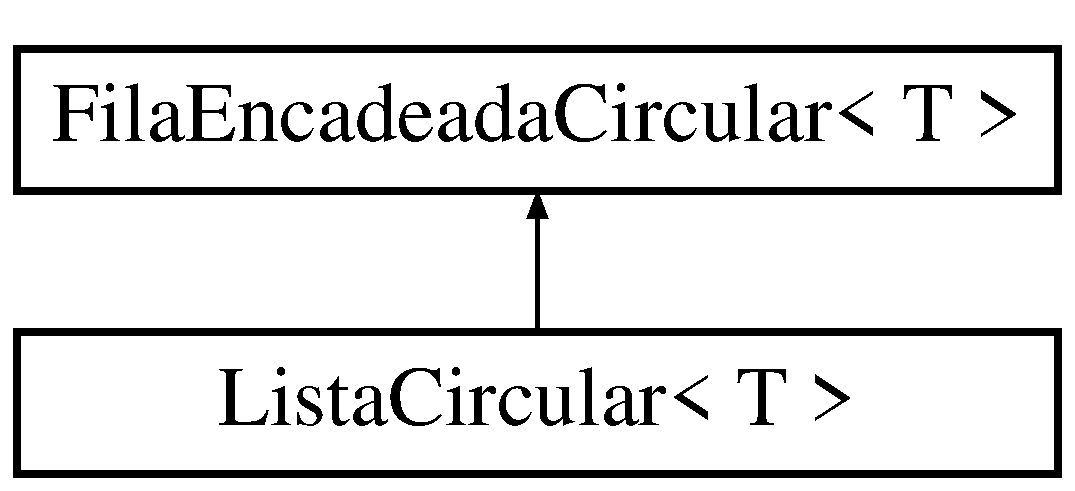
\includegraphics[height=2.000000cm]{class_fila_encadeada_circular}
\end{center}
\end{figure}
\subsection*{Membros públicos}
\begin{DoxyCompactItemize}
\item 
\hyperlink{class_fila_encadeada_circular_abc8c9843469e21051da2301482607eee}{Fila\+Encadeada\+Circular} ()
\item 
\hyperlink{class_fila_encadeada_circular_af0fc66d6ac033bbeed34e605f2aac6f7}{$\sim$\+Fila\+Encadeada\+Circular} ()
\item 
void \hyperlink{class_fila_encadeada_circular_a7cf9350910752a11791a8c11d9f9db6b}{cria\+Estrutura} ()
\item 
bool \hyperlink{class_fila_encadeada_circular_ae3672f48a1ba222f8b763ffdf23b7a28}{estrutura\+Vazia} ()
\item 
int \hyperlink{class_fila_encadeada_circular_a5be1b9cba51f2a0e56ff28cac6ccf95c}{adiciona} (T $\ast$dado)
\item 
T $\ast$ \hyperlink{class_fila_encadeada_circular_a6d92caf9954566984c82317355f1cfea}{retira} ()
\item 
int \hyperlink{class_fila_encadeada_circular_ac8cfb69ffbb7928b635602f323f558ce}{adiciona\+No\+Inicio} (T $\ast$dado)
\item 
T \hyperlink{class_fila_encadeada_circular_a453f5226938097c020a82f24522886e1}{obter\+Topo} ()
\item 
int \hyperlink{class_fila_encadeada_circular_ae58955bcc5f4d14d1f55a40cf39471ec}{obter\+Tamanho} ()
\item 
void \hyperlink{class_fila_encadeada_circular_a9639a74b8534ea1a7c635fa23a9cf284}{destroi\+Estrutura} ()
\end{DoxyCompactItemize}
\subsection*{Atributos Protegidos}
\begin{DoxyCompactItemize}
\item 
\hyperlink{classt_elemento}{t\+Elemento}$<$ T $>$ $\ast$ \hyperlink{class_fila_encadeada_circular_a4286760de29b4691846e8fef53459f33}{sentinela}
\item 
int \hyperlink{class_fila_encadeada_circular_a681be4fb4159df86faab4421fcacb099}{tamanho}
\end{DoxyCompactItemize}


\subsection{Documentação dos Construtores \& Destrutor}
\hypertarget{class_fila_encadeada_circular_abc8c9843469e21051da2301482607eee}{\index{Fila\+Encadeada\+Circular@{Fila\+Encadeada\+Circular}!Fila\+Encadeada\+Circular@{Fila\+Encadeada\+Circular}}
\index{Fila\+Encadeada\+Circular@{Fila\+Encadeada\+Circular}!Fila\+Encadeada\+Circular@{Fila\+Encadeada\+Circular}}
\subsubsection[{Fila\+Encadeada\+Circular}]{\setlength{\rightskip}{0pt plus 5cm}template$<$class T$>$ {\bf Fila\+Encadeada\+Circular}$<$ T $>$\+::{\bf Fila\+Encadeada\+Circular} (
\begin{DoxyParamCaption}
{}
\end{DoxyParamCaption}
)\hspace{0.3cm}{\ttfamily [inline]}}}\label{class_fila_encadeada_circular_abc8c9843469e21051da2301482607eee}
\hypertarget{class_fila_encadeada_circular_af0fc66d6ac033bbeed34e605f2aac6f7}{\index{Fila\+Encadeada\+Circular@{Fila\+Encadeada\+Circular}!````~Fila\+Encadeada\+Circular@{$\sim$\+Fila\+Encadeada\+Circular}}
\index{````~Fila\+Encadeada\+Circular@{$\sim$\+Fila\+Encadeada\+Circular}!Fila\+Encadeada\+Circular@{Fila\+Encadeada\+Circular}}
\subsubsection[{$\sim$\+Fila\+Encadeada\+Circular}]{\setlength{\rightskip}{0pt plus 5cm}template$<$class T$>$ {\bf Fila\+Encadeada\+Circular}$<$ T $>$\+::$\sim${\bf Fila\+Encadeada\+Circular} (
\begin{DoxyParamCaption}
{}
\end{DoxyParamCaption}
)\hspace{0.3cm}{\ttfamily [inline]}}}\label{class_fila_encadeada_circular_af0fc66d6ac033bbeed34e605f2aac6f7}


\subsection{Documentação dos métodos}
\hypertarget{class_fila_encadeada_circular_a5be1b9cba51f2a0e56ff28cac6ccf95c}{\index{Fila\+Encadeada\+Circular@{Fila\+Encadeada\+Circular}!adiciona@{adiciona}}
\index{adiciona@{adiciona}!Fila\+Encadeada\+Circular@{Fila\+Encadeada\+Circular}}
\subsubsection[{adiciona}]{\setlength{\rightskip}{0pt plus 5cm}template$<$class T$>$ int {\bf Fila\+Encadeada\+Circular}$<$ T $>$\+::adiciona (
\begin{DoxyParamCaption}
\item[{T $\ast$}]{dado}
\end{DoxyParamCaption}
)\hspace{0.3cm}{\ttfamily [inline]}}}\label{class_fila_encadeada_circular_a5be1b9cba51f2a0e56ff28cac6ccf95c}
Adiciona um novo elemento no final da estrutura \hypertarget{class_fila_encadeada_circular_ac8cfb69ffbb7928b635602f323f558ce}{\index{Fila\+Encadeada\+Circular@{Fila\+Encadeada\+Circular}!adiciona\+No\+Inicio@{adiciona\+No\+Inicio}}
\index{adiciona\+No\+Inicio@{adiciona\+No\+Inicio}!Fila\+Encadeada\+Circular@{Fila\+Encadeada\+Circular}}
\subsubsection[{adiciona\+No\+Inicio}]{\setlength{\rightskip}{0pt plus 5cm}template$<$class T$>$ int {\bf Fila\+Encadeada\+Circular}$<$ T $>$\+::adiciona\+No\+Inicio (
\begin{DoxyParamCaption}
\item[{T $\ast$}]{dado}
\end{DoxyParamCaption}
)\hspace{0.3cm}{\ttfamily [inline]}}}\label{class_fila_encadeada_circular_ac8cfb69ffbb7928b635602f323f558ce}
Adiciona um novo elemento no início da estrutura \hypertarget{class_fila_encadeada_circular_a7cf9350910752a11791a8c11d9f9db6b}{\index{Fila\+Encadeada\+Circular@{Fila\+Encadeada\+Circular}!cria\+Estrutura@{cria\+Estrutura}}
\index{cria\+Estrutura@{cria\+Estrutura}!Fila\+Encadeada\+Circular@{Fila\+Encadeada\+Circular}}
\subsubsection[{cria\+Estrutura}]{\setlength{\rightskip}{0pt plus 5cm}template$<$class T$>$ void {\bf Fila\+Encadeada\+Circular}$<$ T $>$\+::cria\+Estrutura (
\begin{DoxyParamCaption}
{}
\end{DoxyParamCaption}
)\hspace{0.3cm}{\ttfamily [inline]}}}\label{class_fila_encadeada_circular_a7cf9350910752a11791a8c11d9f9db6b}
Inicialização da estrutura \hypertarget{class_fila_encadeada_circular_a9639a74b8534ea1a7c635fa23a9cf284}{\index{Fila\+Encadeada\+Circular@{Fila\+Encadeada\+Circular}!destroi\+Estrutura@{destroi\+Estrutura}}
\index{destroi\+Estrutura@{destroi\+Estrutura}!Fila\+Encadeada\+Circular@{Fila\+Encadeada\+Circular}}
\subsubsection[{destroi\+Estrutura}]{\setlength{\rightskip}{0pt plus 5cm}template$<$class T$>$ void {\bf Fila\+Encadeada\+Circular}$<$ T $>$\+::destroi\+Estrutura (
\begin{DoxyParamCaption}
{}
\end{DoxyParamCaption}
)\hspace{0.3cm}{\ttfamily [inline]}}}\label{class_fila_encadeada_circular_a9639a74b8534ea1a7c635fa23a9cf284}
Reinicializa a estrutura \hypertarget{class_fila_encadeada_circular_ae3672f48a1ba222f8b763ffdf23b7a28}{\index{Fila\+Encadeada\+Circular@{Fila\+Encadeada\+Circular}!estrutura\+Vazia@{estrutura\+Vazia}}
\index{estrutura\+Vazia@{estrutura\+Vazia}!Fila\+Encadeada\+Circular@{Fila\+Encadeada\+Circular}}
\subsubsection[{estrutura\+Vazia}]{\setlength{\rightskip}{0pt plus 5cm}template$<$class T$>$ bool {\bf Fila\+Encadeada\+Circular}$<$ T $>$\+::estrutura\+Vazia (
\begin{DoxyParamCaption}
{}
\end{DoxyParamCaption}
)\hspace{0.3cm}{\ttfamily [inline]}}}\label{class_fila_encadeada_circular_ae3672f48a1ba222f8b763ffdf23b7a28}
Retorna se a estrutura encontra-\/se vazia \hypertarget{class_fila_encadeada_circular_ae58955bcc5f4d14d1f55a40cf39471ec}{\index{Fila\+Encadeada\+Circular@{Fila\+Encadeada\+Circular}!obter\+Tamanho@{obter\+Tamanho}}
\index{obter\+Tamanho@{obter\+Tamanho}!Fila\+Encadeada\+Circular@{Fila\+Encadeada\+Circular}}
\subsubsection[{obter\+Tamanho}]{\setlength{\rightskip}{0pt plus 5cm}template$<$class T$>$ int {\bf Fila\+Encadeada\+Circular}$<$ T $>$\+::obter\+Tamanho (
\begin{DoxyParamCaption}
{}
\end{DoxyParamCaption}
)\hspace{0.3cm}{\ttfamily [inline]}}}\label{class_fila_encadeada_circular_ae58955bcc5f4d14d1f55a40cf39471ec}
Retorna o tamanho da estrutura \hypertarget{class_fila_encadeada_circular_a453f5226938097c020a82f24522886e1}{\index{Fila\+Encadeada\+Circular@{Fila\+Encadeada\+Circular}!obter\+Topo@{obter\+Topo}}
\index{obter\+Topo@{obter\+Topo}!Fila\+Encadeada\+Circular@{Fila\+Encadeada\+Circular}}
\subsubsection[{obter\+Topo}]{\setlength{\rightskip}{0pt plus 5cm}template$<$class T$>$ T {\bf Fila\+Encadeada\+Circular}$<$ T $>$\+::obter\+Topo (
\begin{DoxyParamCaption}
{}
\end{DoxyParamCaption}
)\hspace{0.3cm}{\ttfamily [inline]}}}\label{class_fila_encadeada_circular_a453f5226938097c020a82f24522886e1}
Retorna o elemento no topo da estrutura \hypertarget{class_fila_encadeada_circular_a6d92caf9954566984c82317355f1cfea}{\index{Fila\+Encadeada\+Circular@{Fila\+Encadeada\+Circular}!retira@{retira}}
\index{retira@{retira}!Fila\+Encadeada\+Circular@{Fila\+Encadeada\+Circular}}
\subsubsection[{retira}]{\setlength{\rightskip}{0pt plus 5cm}template$<$class T$>$ T$\ast$ {\bf Fila\+Encadeada\+Circular}$<$ T $>$\+::retira (
\begin{DoxyParamCaption}
{}
\end{DoxyParamCaption}
)\hspace{0.3cm}{\ttfamily [inline]}}}\label{class_fila_encadeada_circular_a6d92caf9954566984c82317355f1cfea}
Remove o primeiro elemento adiciona na estrutura 

\subsection{Documentação dos dados membro}
\hypertarget{class_fila_encadeada_circular_a4286760de29b4691846e8fef53459f33}{\index{Fila\+Encadeada\+Circular@{Fila\+Encadeada\+Circular}!sentinela@{sentinela}}
\index{sentinela@{sentinela}!Fila\+Encadeada\+Circular@{Fila\+Encadeada\+Circular}}
\subsubsection[{sentinela}]{\setlength{\rightskip}{0pt plus 5cm}template$<$class T$>$ {\bf t\+Elemento}$<$T$>$$\ast$ {\bf Fila\+Encadeada\+Circular}$<$ T $>$\+::sentinela\hspace{0.3cm}{\ttfamily [protected]}}}\label{class_fila_encadeada_circular_a4286760de29b4691846e8fef53459f33}
\hypertarget{class_fila_encadeada_circular_a681be4fb4159df86faab4421fcacb099}{\index{Fila\+Encadeada\+Circular@{Fila\+Encadeada\+Circular}!tamanho@{tamanho}}
\index{tamanho@{tamanho}!Fila\+Encadeada\+Circular@{Fila\+Encadeada\+Circular}}
\subsubsection[{tamanho}]{\setlength{\rightskip}{0pt plus 5cm}template$<$class T$>$ int {\bf Fila\+Encadeada\+Circular}$<$ T $>$\+::tamanho\hspace{0.3cm}{\ttfamily [protected]}}}\label{class_fila_encadeada_circular_a681be4fb4159df86faab4421fcacb099}


A documentação para esta classe foi gerada a partir do seguinte ficheiro\+:\begin{DoxyCompactItemize}
\item 
\hyperlink{_fila_encadeada_8hpp}{Fila\+Encadeada.\+hpp}\end{DoxyCompactItemize}

\hypertarget{class_lista_circular}{\section{Referência à classe Template Lista\+Circular$<$ T $>$}
\label{class_lista_circular}\index{Lista\+Circular$<$ T $>$@{Lista\+Circular$<$ T $>$}}
}


Implementação da estrutura de dado lista circular que herda da classe \hyperlink{class_fila_encadeada_circular}{Fila\+Encadeada\+Circular}.  




{\ttfamily \#include $<$Lista\+Circular.\+hpp$>$}

Diagrama de heranças da classe Lista\+Circular$<$ T $>$\begin{figure}[H]
\begin{center}
\leavevmode
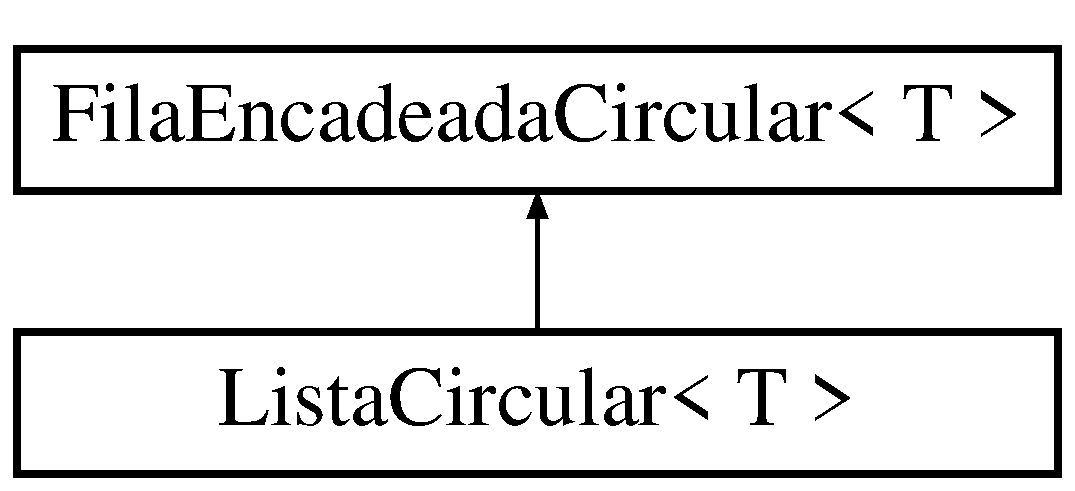
\includegraphics[height=2.000000cm]{class_lista_circular}
\end{center}
\end{figure}
\subsection*{Membros públicos}
\begin{DoxyCompactItemize}
\item 
\hyperlink{class_lista_circular_a257dc7d8b78f8312ac821ba437d9ab77}{Lista\+Circular} ()
\item 
\hyperlink{class_lista_circular_a17151a2a3416edbcdb8d095e64068c05}{$\sim$\+Lista\+Circular} ()
\item 
T $\ast$ \hyperlink{class_lista_circular_ae60601f89f078c8e456e6cd27188ea6d}{retira\+Do\+Inicio} ()
\item 
int \hyperlink{class_lista_circular_affd9b0cb331519a4386dc172708a4729}{adiciona\+No\+Fim} (T $\ast$dado)
\item 
T $\ast$ \hyperlink{class_lista_circular_a5314f5fcd36f0a7bc3f140971737b66a}{retira\+Do\+Fim} ()
\item 
\hyperlink{classt_elemento}{t\+Elemento}$<$ T $>$ $\ast$ \hyperlink{class_lista_circular_abfe109e00fc3bb438a26335586c2e0cb}{obter\+Proximo\+Decrescente} (int posicao)
\item 
\hyperlink{classt_elemento}{t\+Elemento}$<$ T $>$ $\ast$ \hyperlink{class_lista_circular_a3eb9602a4d4585f2b5d8bca3dd66146d}{obter\+Anterior\+Crescente} (int posicao)
\item 
int \hyperlink{class_lista_circular_a8fdef408a651dd0e86ef251ffe58e074}{adiciona\+Na\+Posicao} (T $\ast$info, int posicao)
\item 
T $\ast$ \hyperlink{class_lista_circular_ae310f8ef47da383064c3921bdc50f1c6}{retira\+Da\+Posicao} (int posicao)
\end{DoxyCompactItemize}
\subsection*{Additional Inherited Members}


\subsection{Documentação dos Construtores \& Destrutor}
\hypertarget{class_lista_circular_a257dc7d8b78f8312ac821ba437d9ab77}{\index{Lista\+Circular@{Lista\+Circular}!Lista\+Circular@{Lista\+Circular}}
\index{Lista\+Circular@{Lista\+Circular}!Lista\+Circular@{Lista\+Circular}}
\subsubsection[{Lista\+Circular}]{\setlength{\rightskip}{0pt plus 5cm}template$<$class T$>$ {\bf Lista\+Circular}$<$ T $>$\+::{\bf Lista\+Circular} (
\begin{DoxyParamCaption}
{}
\end{DoxyParamCaption}
)\hspace{0.3cm}{\ttfamily [inline]}}}\label{class_lista_circular_a257dc7d8b78f8312ac821ba437d9ab77}
\hypertarget{class_lista_circular_a17151a2a3416edbcdb8d095e64068c05}{\index{Lista\+Circular@{Lista\+Circular}!````~Lista\+Circular@{$\sim$\+Lista\+Circular}}
\index{````~Lista\+Circular@{$\sim$\+Lista\+Circular}!Lista\+Circular@{Lista\+Circular}}
\subsubsection[{$\sim$\+Lista\+Circular}]{\setlength{\rightskip}{0pt plus 5cm}template$<$class T$>$ {\bf Lista\+Circular}$<$ T $>$\+::$\sim${\bf Lista\+Circular} (
\begin{DoxyParamCaption}
{}
\end{DoxyParamCaption}
)\hspace{0.3cm}{\ttfamily [inline]}}}\label{class_lista_circular_a17151a2a3416edbcdb8d095e64068c05}


\subsection{Documentação dos métodos}
\hypertarget{class_lista_circular_a8fdef408a651dd0e86ef251ffe58e074}{\index{Lista\+Circular@{Lista\+Circular}!adiciona\+Na\+Posicao@{adiciona\+Na\+Posicao}}
\index{adiciona\+Na\+Posicao@{adiciona\+Na\+Posicao}!Lista\+Circular@{Lista\+Circular}}
\subsubsection[{adiciona\+Na\+Posicao}]{\setlength{\rightskip}{0pt plus 5cm}template$<$class T$>$ int {\bf Lista\+Circular}$<$ T $>$\+::adiciona\+Na\+Posicao (
\begin{DoxyParamCaption}
\item[{T $\ast$}]{info, }
\item[{int}]{posicao}
\end{DoxyParamCaption}
)\hspace{0.3cm}{\ttfamily [inline]}}}\label{class_lista_circular_a8fdef408a651dd0e86ef251ffe58e074}
Responsável por adicionar um novo elemento na posição informada \hypertarget{class_lista_circular_affd9b0cb331519a4386dc172708a4729}{\index{Lista\+Circular@{Lista\+Circular}!adiciona\+No\+Fim@{adiciona\+No\+Fim}}
\index{adiciona\+No\+Fim@{adiciona\+No\+Fim}!Lista\+Circular@{Lista\+Circular}}
\subsubsection[{adiciona\+No\+Fim}]{\setlength{\rightskip}{0pt plus 5cm}template$<$class T$>$ int {\bf Lista\+Circular}$<$ T $>$\+::adiciona\+No\+Fim (
\begin{DoxyParamCaption}
\item[{T $\ast$}]{dado}
\end{DoxyParamCaption}
)\hspace{0.3cm}{\ttfamily [inline]}}}\label{class_lista_circular_affd9b0cb331519a4386dc172708a4729}
Responsável por adicionar um novo elemento no fim da fila \hypertarget{class_lista_circular_a3eb9602a4d4585f2b5d8bca3dd66146d}{\index{Lista\+Circular@{Lista\+Circular}!obter\+Anterior\+Crescente@{obter\+Anterior\+Crescente}}
\index{obter\+Anterior\+Crescente@{obter\+Anterior\+Crescente}!Lista\+Circular@{Lista\+Circular}}
\subsubsection[{obter\+Anterior\+Crescente}]{\setlength{\rightskip}{0pt plus 5cm}template$<$class T$>$ {\bf t\+Elemento}$<$T$>$$\ast$ {\bf Lista\+Circular}$<$ T $>$\+::obter\+Anterior\+Crescente (
\begin{DoxyParamCaption}
\item[{int}]{posicao}
\end{DoxyParamCaption}
)\hspace{0.3cm}{\ttfamily [inline]}}}\label{class_lista_circular_a3eb9602a4d4585f2b5d8bca3dd66146d}
Retorna o elemento anterior em ordem crescente (iterando pela direita) \hypertarget{class_lista_circular_abfe109e00fc3bb438a26335586c2e0cb}{\index{Lista\+Circular@{Lista\+Circular}!obter\+Proximo\+Decrescente@{obter\+Proximo\+Decrescente}}
\index{obter\+Proximo\+Decrescente@{obter\+Proximo\+Decrescente}!Lista\+Circular@{Lista\+Circular}}
\subsubsection[{obter\+Proximo\+Decrescente}]{\setlength{\rightskip}{0pt plus 5cm}template$<$class T$>$ {\bf t\+Elemento}$<$T$>$$\ast$ {\bf Lista\+Circular}$<$ T $>$\+::obter\+Proximo\+Decrescente (
\begin{DoxyParamCaption}
\item[{int}]{posicao}
\end{DoxyParamCaption}
)\hspace{0.3cm}{\ttfamily [inline]}}}\label{class_lista_circular_abfe109e00fc3bb438a26335586c2e0cb}
Retorna o proximo elemento em ordem decrescente (iterando pela esquerda) \hypertarget{class_lista_circular_ae310f8ef47da383064c3921bdc50f1c6}{\index{Lista\+Circular@{Lista\+Circular}!retira\+Da\+Posicao@{retira\+Da\+Posicao}}
\index{retira\+Da\+Posicao@{retira\+Da\+Posicao}!Lista\+Circular@{Lista\+Circular}}
\subsubsection[{retira\+Da\+Posicao}]{\setlength{\rightskip}{0pt plus 5cm}template$<$class T$>$ T$\ast$ {\bf Lista\+Circular}$<$ T $>$\+::retira\+Da\+Posicao (
\begin{DoxyParamCaption}
\item[{int}]{posicao}
\end{DoxyParamCaption}
)\hspace{0.3cm}{\ttfamily [inline]}}}\label{class_lista_circular_ae310f8ef47da383064c3921bdc50f1c6}
Responsável por remover um elemento da posição informada \hypertarget{class_lista_circular_a5314f5fcd36f0a7bc3f140971737b66a}{\index{Lista\+Circular@{Lista\+Circular}!retira\+Do\+Fim@{retira\+Do\+Fim}}
\index{retira\+Do\+Fim@{retira\+Do\+Fim}!Lista\+Circular@{Lista\+Circular}}
\subsubsection[{retira\+Do\+Fim}]{\setlength{\rightskip}{0pt plus 5cm}template$<$class T$>$ T$\ast$ {\bf Lista\+Circular}$<$ T $>$\+::retira\+Do\+Fim (
\begin{DoxyParamCaption}
{}
\end{DoxyParamCaption}
)\hspace{0.3cm}{\ttfamily [inline]}}}\label{class_lista_circular_a5314f5fcd36f0a7bc3f140971737b66a}
Responsável por retirar o elemento do fim da fila \hypertarget{class_lista_circular_ae60601f89f078c8e456e6cd27188ea6d}{\index{Lista\+Circular@{Lista\+Circular}!retira\+Do\+Inicio@{retira\+Do\+Inicio}}
\index{retira\+Do\+Inicio@{retira\+Do\+Inicio}!Lista\+Circular@{Lista\+Circular}}
\subsubsection[{retira\+Do\+Inicio}]{\setlength{\rightskip}{0pt plus 5cm}template$<$class T$>$ T$\ast$ {\bf Lista\+Circular}$<$ T $>$\+::retira\+Do\+Inicio (
\begin{DoxyParamCaption}
{}
\end{DoxyParamCaption}
)\hspace{0.3cm}{\ttfamily [inline]}}}\label{class_lista_circular_ae60601f89f078c8e456e6cd27188ea6d}
Responsável por retirar o elemento do inicio da fila 

A documentação para esta classe foi gerada a partir do seguinte ficheiro\+:\begin{DoxyCompactItemize}
\item 
\hyperlink{_lista_circular_8hpp}{Lista\+Circular.\+hpp}\end{DoxyCompactItemize}

\hypertarget{class_supermercado}{\section{Referência à classe Supermercado}
\label{class_supermercado}\index{Supermercado@{Supermercado}}
}


Responsável pelo armazenamento dos parametros de execução e por conter a lógica da aplicação~\newline
 A funcionalidade relacionada com a desistencia de compra pelos clientes não está ocorrendo devido ao parametro padrão definido nos requisitos do projeto ser mutualmente exclusivo com a contratação de novos caixas.  




{\ttfamily \#include $<$Supermercado.\+h$>$}

\subsection*{Membros públicos}
\begin{DoxyCompactItemize}
\item 
\hyperlink{class_supermercado_a51e46aa12924a52dbf0e4f26ad3bd7b3}{Supermercado} (std\+::string nome\+Do\+Supermercado, \hyperlink{class_lista_circular}{Lista\+Circular}$<$ std\+::string $>$ $\ast$identificadores\+Dos\+Caixas, \hyperlink{class_lista_circular}{Lista\+Circular}$<$ \hyperlink{class_caixa_a0e98d0cd8dc2ff4f73d637d73f7bbe85}{Caixa\+::\+Eficiencia} $>$ $\ast$eficiencia\+Dos\+Caixas, \hyperlink{class_lista_circular}{Lista\+Circular}$<$ double $>$ $\ast$salarios\+Dos\+Caixas, int tempo\+Medio\+Em\+Segundos\+De\+Chegada\+De\+Novos\+Clientes, int tempo\+Total\+De\+Simulacao\+Em\+Horas, int tamanho\+Maximo\+Das\+Filas\+Para\+Desistir)
\item 
\hyperlink{class_supermercado_a3f0598a98bd6179c4553eb213c4aa48c}{Supermercado} (std\+::string caminho\+Arquivo\+Configuracao)
\item 
\hyperlink{class_supermercado_ab21737ada65202c6293a503bfa64e8a0}{$\sim$\+Supermercado} (void)
\item 
void \hyperlink{class_supermercado_a2244eb3e925e1e5e78a0d152bbaa78a9}{rodar\+Simulacao} ()
\end{DoxyCompactItemize}


\subsection{Documentação dos Construtores \& Destrutor}
\hypertarget{class_supermercado_a51e46aa12924a52dbf0e4f26ad3bd7b3}{\index{Supermercado@{Supermercado}!Supermercado@{Supermercado}}
\index{Supermercado@{Supermercado}!Supermercado@{Supermercado}}
\subsubsection[{Supermercado}]{\setlength{\rightskip}{0pt plus 5cm}Supermercado\+::\+Supermercado (
\begin{DoxyParamCaption}
\item[{std\+::string}]{nome\+Do\+Supermercado, }
\item[{{\bf Lista\+Circular}$<$ std\+::string $>$ $\ast$}]{identificadores\+Dos\+Caixas, }
\item[{{\bf Lista\+Circular}$<$ {\bf Caixa\+::\+Eficiencia} $>$ $\ast$}]{eficiencia\+Dos\+Caixas, }
\item[{{\bf Lista\+Circular}$<$ double $>$ $\ast$}]{salarios\+Dos\+Caixas, }
\item[{int}]{tempo\+Medio\+Em\+Segundos\+De\+Chegada\+De\+Novos\+Clientes, }
\item[{int}]{tempo\+Total\+De\+Simulacao\+Em\+Horas, }
\item[{int}]{tamanho\+Maximo\+Das\+Filas\+Para\+Desistir}
\end{DoxyParamCaption}
)}}\label{class_supermercado_a51e46aa12924a52dbf0e4f26ad3bd7b3}

\begin{DoxyParams}{Parâmetros}
{\em tamanho\+Maximo\+Das\+Filas\+Para\+Desistir} & Quando todos os caixas estiverem com esse numero de clientes na fila e um novo cliente chegar este desiste da compra. \\
\hline
\end{DoxyParams}
\hypertarget{class_supermercado_a3f0598a98bd6179c4553eb213c4aa48c}{\index{Supermercado@{Supermercado}!Supermercado@{Supermercado}}
\index{Supermercado@{Supermercado}!Supermercado@{Supermercado}}
\subsubsection[{Supermercado}]{\setlength{\rightskip}{0pt plus 5cm}Supermercado\+::\+Supermercado (
\begin{DoxyParamCaption}
\item[{std\+::string}]{caminho\+Arquivo\+Configuracao}
\end{DoxyParamCaption}
)}}\label{class_supermercado_a3f0598a98bd6179c4553eb213c4aa48c}
Construtor que recebe o arquivo de configuração de onde os parametros serão extraidos \hypertarget{class_supermercado_ab21737ada65202c6293a503bfa64e8a0}{\index{Supermercado@{Supermercado}!````~Supermercado@{$\sim$\+Supermercado}}
\index{````~Supermercado@{$\sim$\+Supermercado}!Supermercado@{Supermercado}}
\subsubsection[{$\sim$\+Supermercado}]{\setlength{\rightskip}{0pt plus 5cm}Supermercado\+::$\sim$\+Supermercado (
\begin{DoxyParamCaption}
\item[{void}]{}
\end{DoxyParamCaption}
)}}\label{class_supermercado_ab21737ada65202c6293a503bfa64e8a0}


\subsection{Documentação dos métodos}
\hypertarget{class_supermercado_a2244eb3e925e1e5e78a0d152bbaa78a9}{\index{Supermercado@{Supermercado}!rodar\+Simulacao@{rodar\+Simulacao}}
\index{rodar\+Simulacao@{rodar\+Simulacao}!Supermercado@{Supermercado}}
\subsubsection[{rodar\+Simulacao}]{\setlength{\rightskip}{0pt plus 5cm}void Supermercado\+::rodar\+Simulacao (
\begin{DoxyParamCaption}
{}
\end{DoxyParamCaption}
)}}\label{class_supermercado_a2244eb3e925e1e5e78a0d152bbaa78a9}
Método principal responsável por simular o funcionamento do \hyperlink{class_supermercado}{Supermercado} e apresentar as estatísticas no final da execução 

A documentação para esta classe foi gerada a partir dos seguintes ficheiros\+:\begin{DoxyCompactItemize}
\item 
\hyperlink{_supermercado_8h}{Supermercado.\+h}\item 
\hyperlink{_supermercado_8cpp}{Supermercado.\+cpp}\end{DoxyCompactItemize}

\hypertarget{classt_elemento}{\section{Referência à classe Template t\+Elemento$<$ T $>$}
\label{classt_elemento}\index{t\+Elemento$<$ T $>$@{t\+Elemento$<$ T $>$}}
}


Responsável por conter e gerenciar os ponteiros para os próximos e anteriores e para a informação em si de uma estrutura duplamente encadeada.  




{\ttfamily \#include $<$t\+Elemento.\+hpp$>$}

\subsection*{Membros públicos}
\begin{DoxyCompactItemize}
\item 
\hyperlink{classt_elemento_ad8dc84de43eca107440039b37e188de6}{t\+Elemento} ()
\item 
\hyperlink{classt_elemento_a2b83968c3cdf56f521b6faff78068bc8}{$\sim$t\+Elemento} ()
\item 
void \hyperlink{classt_elemento_aa9f5f970a2de51063c78e54229c35867}{set\+Proximo} (\hyperlink{classt_elemento}{t\+Elemento}$<$ T $>$ $\ast$proximo)
\item 
\hyperlink{classt_elemento}{t\+Elemento}$<$ T $>$ $\ast$ \hyperlink{classt_elemento_acfbfbaaedb5a662a999f655c171b50f1}{get\+Proximo} ()
\item 
void \hyperlink{classt_elemento_a484d3f94a793fc00e935a2d442019ac4}{set\+Anterior} (\hyperlink{classt_elemento}{t\+Elemento}$<$ T $>$ $\ast$anterior)
\item 
\hyperlink{classt_elemento}{t\+Elemento}$<$ T $>$ $\ast$ \hyperlink{classt_elemento_a467573ea5ebe5fdd5e5739f62d8ecc7d}{get\+Anterior} ()
\item 
void \hyperlink{classt_elemento_a20c8ed616c72b00387650d06a8368834}{set\+Info} (T $\ast$info)
\item 
T $\ast$ \hyperlink{classt_elemento_af7e39d1f741ccf80a012660530a32e1b}{get\+Info} ()
\end{DoxyCompactItemize}


\subsection{Documentação dos Construtores \& Destrutor}
\hypertarget{classt_elemento_ad8dc84de43eca107440039b37e188de6}{\index{t\+Elemento@{t\+Elemento}!t\+Elemento@{t\+Elemento}}
\index{t\+Elemento@{t\+Elemento}!t\+Elemento@{t\+Elemento}}
\subsubsection[{t\+Elemento}]{\setlength{\rightskip}{0pt plus 5cm}template$<$class T$>$ {\bf t\+Elemento}$<$ T $>$\+::{\bf t\+Elemento} (
\begin{DoxyParamCaption}
{}
\end{DoxyParamCaption}
)\hspace{0.3cm}{\ttfamily [inline]}}}\label{classt_elemento_ad8dc84de43eca107440039b37e188de6}
\hypertarget{classt_elemento_a2b83968c3cdf56f521b6faff78068bc8}{\index{t\+Elemento@{t\+Elemento}!````~t\+Elemento@{$\sim$t\+Elemento}}
\index{````~t\+Elemento@{$\sim$t\+Elemento}!t\+Elemento@{t\+Elemento}}
\subsubsection[{$\sim$t\+Elemento}]{\setlength{\rightskip}{0pt plus 5cm}template$<$class T$>$ {\bf t\+Elemento}$<$ T $>$\+::$\sim${\bf t\+Elemento} (
\begin{DoxyParamCaption}
{}
\end{DoxyParamCaption}
)\hspace{0.3cm}{\ttfamily [inline]}}}\label{classt_elemento_a2b83968c3cdf56f521b6faff78068bc8}


\subsection{Documentação dos métodos}
\hypertarget{classt_elemento_a467573ea5ebe5fdd5e5739f62d8ecc7d}{\index{t\+Elemento@{t\+Elemento}!get\+Anterior@{get\+Anterior}}
\index{get\+Anterior@{get\+Anterior}!t\+Elemento@{t\+Elemento}}
\subsubsection[{get\+Anterior}]{\setlength{\rightskip}{0pt plus 5cm}template$<$class T$>$ {\bf t\+Elemento}$<$T$>$$\ast$ {\bf t\+Elemento}$<$ T $>$\+::get\+Anterior (
\begin{DoxyParamCaption}
{}
\end{DoxyParamCaption}
)\hspace{0.3cm}{\ttfamily [inline]}}}\label{classt_elemento_a467573ea5ebe5fdd5e5739f62d8ecc7d}
Retorna o ponteiro para o elemento anterior a este na estrutura \hypertarget{classt_elemento_af7e39d1f741ccf80a012660530a32e1b}{\index{t\+Elemento@{t\+Elemento}!get\+Info@{get\+Info}}
\index{get\+Info@{get\+Info}!t\+Elemento@{t\+Elemento}}
\subsubsection[{get\+Info}]{\setlength{\rightskip}{0pt plus 5cm}template$<$class T$>$ T$\ast$ {\bf t\+Elemento}$<$ T $>$\+::get\+Info (
\begin{DoxyParamCaption}
{}
\end{DoxyParamCaption}
)\hspace{0.3cm}{\ttfamily [inline]}}}\label{classt_elemento_af7e39d1f741ccf80a012660530a32e1b}
Retorna as informações do elemento \hypertarget{classt_elemento_acfbfbaaedb5a662a999f655c171b50f1}{\index{t\+Elemento@{t\+Elemento}!get\+Proximo@{get\+Proximo}}
\index{get\+Proximo@{get\+Proximo}!t\+Elemento@{t\+Elemento}}
\subsubsection[{get\+Proximo}]{\setlength{\rightskip}{0pt plus 5cm}template$<$class T$>$ {\bf t\+Elemento}$<$T$>$$\ast$ {\bf t\+Elemento}$<$ T $>$\+::get\+Proximo (
\begin{DoxyParamCaption}
{}
\end{DoxyParamCaption}
)\hspace{0.3cm}{\ttfamily [inline]}}}\label{classt_elemento_acfbfbaaedb5a662a999f655c171b50f1}
Retorna o ponteiro para o elemento posterior a este na estrutura \hypertarget{classt_elemento_a484d3f94a793fc00e935a2d442019ac4}{\index{t\+Elemento@{t\+Elemento}!set\+Anterior@{set\+Anterior}}
\index{set\+Anterior@{set\+Anterior}!t\+Elemento@{t\+Elemento}}
\subsubsection[{set\+Anterior}]{\setlength{\rightskip}{0pt plus 5cm}template$<$class T$>$ void {\bf t\+Elemento}$<$ T $>$\+::set\+Anterior (
\begin{DoxyParamCaption}
\item[{{\bf t\+Elemento}$<$ T $>$ $\ast$}]{anterior}
\end{DoxyParamCaption}
)\hspace{0.3cm}{\ttfamily [inline]}}}\label{classt_elemento_a484d3f94a793fc00e935a2d442019ac4}
Responsável por definir o ponteiro para o elemento anterior a este na estrutura \hypertarget{classt_elemento_a20c8ed616c72b00387650d06a8368834}{\index{t\+Elemento@{t\+Elemento}!set\+Info@{set\+Info}}
\index{set\+Info@{set\+Info}!t\+Elemento@{t\+Elemento}}
\subsubsection[{set\+Info}]{\setlength{\rightskip}{0pt plus 5cm}template$<$class T$>$ void {\bf t\+Elemento}$<$ T $>$\+::set\+Info (
\begin{DoxyParamCaption}
\item[{T $\ast$}]{info}
\end{DoxyParamCaption}
)\hspace{0.3cm}{\ttfamily [inline]}}}\label{classt_elemento_a20c8ed616c72b00387650d06a8368834}
Responsável por definir o ponteiro para o as informações do elemento \hypertarget{classt_elemento_aa9f5f970a2de51063c78e54229c35867}{\index{t\+Elemento@{t\+Elemento}!set\+Proximo@{set\+Proximo}}
\index{set\+Proximo@{set\+Proximo}!t\+Elemento@{t\+Elemento}}
\subsubsection[{set\+Proximo}]{\setlength{\rightskip}{0pt plus 5cm}template$<$class T$>$ void {\bf t\+Elemento}$<$ T $>$\+::set\+Proximo (
\begin{DoxyParamCaption}
\item[{{\bf t\+Elemento}$<$ T $>$ $\ast$}]{proximo}
\end{DoxyParamCaption}
)\hspace{0.3cm}{\ttfamily [inline]}}}\label{classt_elemento_aa9f5f970a2de51063c78e54229c35867}
Responsável por definir o ponteiro para o elemento posterior a este na estrutura 

A documentação para esta classe foi gerada a partir do seguinte ficheiro\+:\begin{DoxyCompactItemize}
\item 
\hyperlink{t_elemento_8hpp}{t\+Elemento.\+hpp}\end{DoxyCompactItemize}

\chapter{Documentação do ficheiro}
\hypertarget{_caixa_8cpp}{\section{Referência ao ficheiro Caixa.\+cpp}
\label{_caixa_8cpp}\index{Caixa.\+cpp@{Caixa.\+cpp}}
}
{\ttfamily \#include \char`\"{}Std\+Afx.\+h\char`\"{}}\\*
{\ttfamily \#include \char`\"{}Caixa.\+h\char`\"{}}\\*
{\ttfamily \#include $<$string.\+h$>$}\\*

\hypertarget{_caixa_8h}{\section{Referência ao ficheiro Caixa.\+h}
\label{_caixa_8h}\index{Caixa.\+h@{Caixa.\+h}}
}
{\ttfamily \#include \char`\"{}Cliente.\+h\char`\"{}}\\*
{\ttfamily \#include \char`\"{}Fila\+Encadeada.\+hpp\char`\"{}}\\*
{\ttfamily \#include $<$string$>$}\\*
\subsection*{Componentes}
\begin{DoxyCompactItemize}
\item 
class \hyperlink{class_caixa}{Caixa}
\begin{DoxyCompactList}\small\item\em Representa um caixa de supermercado. \end{DoxyCompactList}\end{DoxyCompactItemize}

\hypertarget{_cliente_8cpp}{\section{Referência ao ficheiro Cliente.\+cpp}
\label{_cliente_8cpp}\index{Cliente.\+cpp@{Cliente.\+cpp}}
}
{\ttfamily \#include \char`\"{}Std\+Afx.\+h\char`\"{}}\\*
{\ttfamily \#include \char`\"{}Cliente.\+h\char`\"{}}\\*
{\ttfamily \#include \char`\"{}Gerador\+Randomico.\+h\char`\"{}}\\*

\hypertarget{_cliente_8h}{\section{Referência ao ficheiro Cliente.\+h}
\label{_cliente_8h}\index{Cliente.\+h@{Cliente.\+h}}
}
{\ttfamily \#include \char`\"{}Lista\+Circular.\+hpp\char`\"{}}\\*
\subsection*{Componentes}
\begin{DoxyCompactItemize}
\item 
class \hyperlink{class_cliente}{Cliente}
\begin{DoxyCompactList}\small\item\em Representa um cliente de supermercado. \end{DoxyCompactList}\end{DoxyCompactItemize}

\hypertarget{_fila_encadeada_8hpp}{\section{Referência ao ficheiro Fila\+Encadeada.\+hpp}
\label{_fila_encadeada_8hpp}\index{Fila\+Encadeada.\+hpp@{Fila\+Encadeada.\+hpp}}
}
{\ttfamily \#include $<$stdlib.\+h$>$}\\*
{\ttfamily \#include $<$stdexcept$>$}\\*
{\ttfamily \#include \char`\"{}t\+Elemento.\+hpp\char`\"{}}\\*
\subsection*{Componentes}
\begin{DoxyCompactItemize}
\item 
class \hyperlink{class_fila_encadeada_circular}{Fila\+Encadeada\+Circular$<$ T $>$}
\begin{DoxyCompactList}\small\item\em Implementação da estrutura de dado fila encadeada circular. \end{DoxyCompactList}\end{DoxyCompactItemize}
\subsection*{Macros}
\begin{DoxyCompactItemize}
\item 
\#define \hyperlink{_fila_encadeada_8hpp_a954d131665f170b5f0b9ad3083e27599}{E\+R\+R\+O\+L\+I\+S\+T\+A\+C\+H\+E\+I\+A}~-\/1
\item 
\#define \hyperlink{_fila_encadeada_8hpp_ac6a2228a8da72468def0d5cd7c50855c}{E\+R\+R\+O\+L\+I\+S\+T\+A\+V\+A\+Z\+I\+A}~-\/2
\item 
\#define \hyperlink{_fila_encadeada_8hpp_a276133910d00a9e29f3fa4c43b6af705}{E\+R\+R\+O\+P\+O\+S\+I\+C\+A\+O}~-\/3
\end{DoxyCompactItemize}


\subsection{Documentação das macros}
\hypertarget{_fila_encadeada_8hpp_a954d131665f170b5f0b9ad3083e27599}{\index{Fila\+Encadeada.\+hpp@{Fila\+Encadeada.\+hpp}!E\+R\+R\+O\+L\+I\+S\+T\+A\+C\+H\+E\+I\+A@{E\+R\+R\+O\+L\+I\+S\+T\+A\+C\+H\+E\+I\+A}}
\index{E\+R\+R\+O\+L\+I\+S\+T\+A\+C\+H\+E\+I\+A@{E\+R\+R\+O\+L\+I\+S\+T\+A\+C\+H\+E\+I\+A}!Fila\+Encadeada.\+hpp@{Fila\+Encadeada.\+hpp}}
\subsubsection[{E\+R\+R\+O\+L\+I\+S\+T\+A\+C\+H\+E\+I\+A}]{\setlength{\rightskip}{0pt plus 5cm}\#define E\+R\+R\+O\+L\+I\+S\+T\+A\+C\+H\+E\+I\+A~-\/1}}\label{_fila_encadeada_8hpp_a954d131665f170b5f0b9ad3083e27599}
\hypertarget{_fila_encadeada_8hpp_ac6a2228a8da72468def0d5cd7c50855c}{\index{Fila\+Encadeada.\+hpp@{Fila\+Encadeada.\+hpp}!E\+R\+R\+O\+L\+I\+S\+T\+A\+V\+A\+Z\+I\+A@{E\+R\+R\+O\+L\+I\+S\+T\+A\+V\+A\+Z\+I\+A}}
\index{E\+R\+R\+O\+L\+I\+S\+T\+A\+V\+A\+Z\+I\+A@{E\+R\+R\+O\+L\+I\+S\+T\+A\+V\+A\+Z\+I\+A}!Fila\+Encadeada.\+hpp@{Fila\+Encadeada.\+hpp}}
\subsubsection[{E\+R\+R\+O\+L\+I\+S\+T\+A\+V\+A\+Z\+I\+A}]{\setlength{\rightskip}{0pt plus 5cm}\#define E\+R\+R\+O\+L\+I\+S\+T\+A\+V\+A\+Z\+I\+A~-\/2}}\label{_fila_encadeada_8hpp_ac6a2228a8da72468def0d5cd7c50855c}
\hypertarget{_fila_encadeada_8hpp_a276133910d00a9e29f3fa4c43b6af705}{\index{Fila\+Encadeada.\+hpp@{Fila\+Encadeada.\+hpp}!E\+R\+R\+O\+P\+O\+S\+I\+C\+A\+O@{E\+R\+R\+O\+P\+O\+S\+I\+C\+A\+O}}
\index{E\+R\+R\+O\+P\+O\+S\+I\+C\+A\+O@{E\+R\+R\+O\+P\+O\+S\+I\+C\+A\+O}!Fila\+Encadeada.\+hpp@{Fila\+Encadeada.\+hpp}}
\subsubsection[{E\+R\+R\+O\+P\+O\+S\+I\+C\+A\+O}]{\setlength{\rightskip}{0pt plus 5cm}\#define E\+R\+R\+O\+P\+O\+S\+I\+C\+A\+O~-\/3}}\label{_fila_encadeada_8hpp_a276133910d00a9e29f3fa4c43b6af705}

\hypertarget{_gerador_randomico_8h}{\section{Referência ao ficheiro Gerador\+Randomico.\+h}
\label{_gerador_randomico_8h}\index{Gerador\+Randomico.\+h@{Gerador\+Randomico.\+h}}
}
{\ttfamily \#include $<$stdlib.\+h$>$}\\*
\subsection*{Funções}
\begin{DoxyCompactItemize}
\item 
double \hyperlink{_gerador_randomico_8h_ac291e880c5395ed90e3306b7344e46ba}{randomico} ()
\end{DoxyCompactItemize}


\subsection{Documentação das funções}
\hypertarget{_gerador_randomico_8h_ac291e880c5395ed90e3306b7344e46ba}{\index{Gerador\+Randomico.\+h@{Gerador\+Randomico.\+h}!randomico@{randomico}}
\index{randomico@{randomico}!Gerador\+Randomico.\+h@{Gerador\+Randomico.\+h}}
\subsubsection[{randomico}]{\setlength{\rightskip}{0pt plus 5cm}double randomico (
\begin{DoxyParamCaption}
{}
\end{DoxyParamCaption}
)\hspace{0.3cm}{\ttfamily [inline]}}}\label{_gerador_randomico_8h_ac291e880c5395ed90e3306b7344e46ba}
Gera um numero randômico entre 0 e 1 usando srand e rand 
\hypertarget{_lista_circular_8hpp}{\section{Referência ao ficheiro Lista\+Circular.\+hpp}
\label{_lista_circular_8hpp}\index{Lista\+Circular.\+hpp@{Lista\+Circular.\+hpp}}
}
{\ttfamily \#include $<$stdlib.\+h$>$}\\*
{\ttfamily \#include $<$stdexcept$>$}\\*
{\ttfamily \#include \char`\"{}t\+Elemento.\+hpp\char`\"{}}\\*
{\ttfamily \#include \char`\"{}Fila\+Encadeada.\+hpp\char`\"{}}\\*
\subsection*{Componentes}
\begin{DoxyCompactItemize}
\item 
class \hyperlink{class_lista_circular}{Lista\+Circular$<$ T $>$}
\begin{DoxyCompactList}\small\item\em Implementação da estrutura de dado lista circular que herda da classe \hyperlink{class_fila_encadeada_circular}{Fila\+Encadeada\+Circular}. \end{DoxyCompactList}\end{DoxyCompactItemize}

\hypertarget{main_8cpp}{\section{Referência ao ficheiro main.\+cpp}
\label{main_8cpp}\index{main.\+cpp@{main.\+cpp}}
}
{\ttfamily \#include $<$iostream$>$}\\*
\subsection*{Funções}
\begin{DoxyCompactItemize}
\item 
int \hyperlink{main_8cpp_ae66f6b31b5ad750f1fe042a706a4e3d4}{main} ()
\end{DoxyCompactItemize}


\subsection{Documentação das funções}
\hypertarget{main_8cpp_ae66f6b31b5ad750f1fe042a706a4e3d4}{\index{main.\+cpp@{main.\+cpp}!main@{main}}
\index{main@{main}!main.\+cpp@{main.\+cpp}}
\subsubsection[{main}]{\setlength{\rightskip}{0pt plus 5cm}int main (
\begin{DoxyParamCaption}
{}
\end{DoxyParamCaption}
)}}\label{main_8cpp_ae66f6b31b5ad750f1fe042a706a4e3d4}

\hypertarget{main_supermercado_8cpp}{\section{Referência ao ficheiro main\+Supermercado.\+cpp}
\label{main_supermercado_8cpp}\index{main\+Supermercado.\+cpp@{main\+Supermercado.\+cpp}}
}
{\ttfamily \#include \char`\"{}stdafx.\+h\char`\"{}}\\*
{\ttfamily \#include \char`\"{}Supermercado.\+h\char`\"{}}\\*
{\ttfamily \#include $<$string$>$}\\*
{\ttfamily \#include $<$ctime$>$}\\*
{\ttfamily \#include $<$iostream$>$}\\*
{\ttfamily \#include $<$fstream$>$}\\*
\subsection*{Funções}
\begin{DoxyCompactItemize}
\item 
int \hyperlink{main_supermercado_8cpp_a0f9d8e9e69f8acdc045770af7e4967e2}{tratar\+Entrada\+Numero} (bool eficiencia=false)
\item 
bool \hyperlink{main_supermercado_8cpp_acded16fadf30198925f82e8a7d1474c5}{arquivo\+Existe} (const std\+::string \&nome\+Arquivo)
\item 
void \hyperlink{main_supermercado_8cpp_af328b9af57d3fc634bd659441e25a3fa}{menu} (\hyperlink{class_supermercado}{Supermercado} $\ast$$\ast$mercado)
\item 
int \hyperlink{main_supermercado_8cpp_ae66f6b31b5ad750f1fe042a706a4e3d4}{main} ()
\end{DoxyCompactItemize}


\subsection{Documentação das funções}
\hypertarget{main_supermercado_8cpp_acded16fadf30198925f82e8a7d1474c5}{\index{main\+Supermercado.\+cpp@{main\+Supermercado.\+cpp}!arquivo\+Existe@{arquivo\+Existe}}
\index{arquivo\+Existe@{arquivo\+Existe}!main\+Supermercado.\+cpp@{main\+Supermercado.\+cpp}}
\subsubsection[{arquivo\+Existe}]{\setlength{\rightskip}{0pt plus 5cm}bool arquivo\+Existe (
\begin{DoxyParamCaption}
\item[{const std\+::string \&}]{nome\+Arquivo}
\end{DoxyParamCaption}
)\hspace{0.3cm}{\ttfamily [inline]}}}\label{main_supermercado_8cpp_acded16fadf30198925f82e8a7d1474c5}
\hypertarget{main_supermercado_8cpp_ae66f6b31b5ad750f1fe042a706a4e3d4}{\index{main\+Supermercado.\+cpp@{main\+Supermercado.\+cpp}!main@{main}}
\index{main@{main}!main\+Supermercado.\+cpp@{main\+Supermercado.\+cpp}}
\subsubsection[{main}]{\setlength{\rightskip}{0pt plus 5cm}int main (
\begin{DoxyParamCaption}
{}
\end{DoxyParamCaption}
)}}\label{main_supermercado_8cpp_ae66f6b31b5ad750f1fe042a706a4e3d4}
\hypertarget{main_supermercado_8cpp_af328b9af57d3fc634bd659441e25a3fa}{\index{main\+Supermercado.\+cpp@{main\+Supermercado.\+cpp}!menu@{menu}}
\index{menu@{menu}!main\+Supermercado.\+cpp@{main\+Supermercado.\+cpp}}
\subsubsection[{menu}]{\setlength{\rightskip}{0pt plus 5cm}void menu (
\begin{DoxyParamCaption}
\item[{{\bf Supermercado} $\ast$$\ast$}]{mercado}
\end{DoxyParamCaption}
)}}\label{main_supermercado_8cpp_af328b9af57d3fc634bd659441e25a3fa}
\hypertarget{main_supermercado_8cpp_a0f9d8e9e69f8acdc045770af7e4967e2}{\index{main\+Supermercado.\+cpp@{main\+Supermercado.\+cpp}!tratar\+Entrada\+Numero@{tratar\+Entrada\+Numero}}
\index{tratar\+Entrada\+Numero@{tratar\+Entrada\+Numero}!main\+Supermercado.\+cpp@{main\+Supermercado.\+cpp}}
\subsubsection[{tratar\+Entrada\+Numero}]{\setlength{\rightskip}{0pt plus 5cm}int tratar\+Entrada\+Numero (
\begin{DoxyParamCaption}
\item[{bool}]{eficiencia = {\ttfamily false}}
\end{DoxyParamCaption}
)}}\label{main_supermercado_8cpp_a0f9d8e9e69f8acdc045770af7e4967e2}

\hypertarget{stdafx_8cpp}{\section{Referência ao ficheiro stdafx.\+cpp}
\label{stdafx_8cpp}\index{stdafx.\+cpp@{stdafx.\+cpp}}
}
{\ttfamily \#include \char`\"{}stdafx.\+h\char`\"{}}\\*

\hypertarget{stdafx_8h}{\section{Referência ao ficheiro stdafx.\+h}
\label{stdafx_8h}\index{stdafx.\+h@{stdafx.\+h}}
}
{\ttfamily \#include \char`\"{}targetver.\+h\char`\"{}}\\*
{\ttfamily \#include $<$stdio.\+h$>$}\\*
{\ttfamily \#include $<$tchar.\+h$>$}\\*

\hypertarget{_supermercado_8cpp}{\section{Referência ao ficheiro Supermercado.\+cpp}
\label{_supermercado_8cpp}\index{Supermercado.\+cpp@{Supermercado.\+cpp}}
}
{\ttfamily \#include \char`\"{}Std\+Afx.\+h\char`\"{}}\\*
{\ttfamily \#include \char`\"{}Supermercado.\+h\char`\"{}}\\*
{\ttfamily \#include \char`\"{}Gerador\+Randomico.\+h\char`\"{}}\\*
{\ttfamily \#include $<$fstream$>$}\\*
{\ttfamily \#include $<$iostream$>$}\\*
{\ttfamily \#include $<$string$>$}\\*
{\ttfamily \#include $<$vector$>$}\\*
\subsection*{Funções}
\begin{DoxyCompactItemize}
\item 
std\+::vector$<$ std\+::string $>$ \hyperlink{_supermercado_8cpp_a0017300954412b8b41d554f20979c23f}{split\+String} (std\+::string original, char delimitador)
\end{DoxyCompactItemize}


\subsection{Documentação das funções}
\hypertarget{_supermercado_8cpp_a0017300954412b8b41d554f20979c23f}{\index{Supermercado.\+cpp@{Supermercado.\+cpp}!split\+String@{split\+String}}
\index{split\+String@{split\+String}!Supermercado.\+cpp@{Supermercado.\+cpp}}
\subsubsection[{split\+String}]{\setlength{\rightskip}{0pt plus 5cm}std\+::vector$<$std\+::string$>$ split\+String (
\begin{DoxyParamCaption}
\item[{std\+::string}]{original, }
\item[{char}]{delimitador}
\end{DoxyParamCaption}
)}}\label{_supermercado_8cpp_a0017300954412b8b41d554f20979c23f}

\hypertarget{_supermercado_8h}{\section{Referência ao ficheiro Supermercado.\+h}
\label{_supermercado_8h}\index{Supermercado.\+h@{Supermercado.\+h}}
}
{\ttfamily \#include \char`\"{}Caixa.\+h\char`\"{}}\\*
{\ttfamily \#include \char`\"{}Lista\+Circular.\+hpp\char`\"{}}\\*
\subsection*{Componentes}
\begin{DoxyCompactItemize}
\item 
class \hyperlink{class_supermercado}{Supermercado}
\begin{DoxyCompactList}\small\item\em Responsável pelo armazenamento dos parametros de execução e por conter a lógica da aplicação~\newline
 A funcionalidade relacionada com a desistencia de compra pelos clientes não está ocorrendo devido ao parametro padrão definido nos requisitos do projeto ser mutualmente exclusivo com a contratação de novos caixas. \end{DoxyCompactList}\end{DoxyCompactItemize}

\hypertarget{targetver_8h}{\section{Referência ao ficheiro targetver.\+h}
\label{targetver_8h}\index{targetver.\+h@{targetver.\+h}}
}
{\ttfamily \#include $<$S\+D\+K\+D\+D\+K\+Ver.\+h$>$}\\*

\hypertarget{t_elemento_8hpp}{\section{Referência ao ficheiro t\+Elemento.\+hpp}
\label{t_elemento_8hpp}\index{t\+Elemento.\+hpp@{t\+Elemento.\+hpp}}
}
\subsection*{Componentes}
\begin{DoxyCompactItemize}
\item 
class \hyperlink{classt_elemento}{t\+Elemento$<$ T $>$}
\begin{DoxyCompactList}\small\item\em Responsável por conter e gerenciar os ponteiros para os próximos e anteriores e para a informação em si de uma estrutura duplamente encadeada. \end{DoxyCompactList}\end{DoxyCompactItemize}

%--- End generated contents ---

% Index
\newpage
\phantomsection
\addcontentsline{toc}{chapter}{Índice}
\printindex

\end{document}
